\begin{definition}
Relacją dwuargumentową jest zbiór do którego należą pary uporządkowane.
\end{definition}
\begin{remark}
Iloczyn $X\times Y$ jest relacją(pełną) pomiędzy zbiorami $X$ i $Y$ ale także każdy podzbiór iloczynu kartezjańskiego zbiorów $X$ i $Y$ jest relacją, czyli $R\subseteq X\times Y$ jest relacją. 
Zauważmy też, że skoro zbiór pusty jest podzbiorem każdego zbioru to korzystając ze znanej własności iloczynu kartezjańskiego zbiorów jeśli $(\emptyset\subseteq X\wedge\emptyset\subseteq Y)\Rightarrow\emptyset\times\emptyset\subseteq X\times Y$, to zbiór pusty jest relacją. Bo $\emptyset\times\emptyset=\emptyset\subseteq X\times Y$.
Należy podkreślić, że relacja $R$ nie musi być iloczynem kartezjańskim dwóch podzbiorów zbiorów $X$ i $Y$. Tzn., skoro relacja $R$ zawiera się w relacji pełnej pomiędzy $X$ i $Y$ to element $x$ z danej pary uporządkowanej należącej do relacji $R$ może należeć do pewnego zbioru $X_{1}\subseteq X$ i podobnie element $y$ z tej pary może należeć do pewnego zbioru $Y_{1}\subseteq Y$. Wówczas $(x,y)\in X_{1}\times Y_{1}$. Ale elementy $x$ i $y$ z innych par uporządkowanych z relacji $R$ mogą należeć także do innych podzbiorów odpowiednio zbiorów $X$ i $Y$. Tak więc przykładowo $R=X_{1}\times Y_{1}$ jest przypadkiem szczególnym relacji $R\subseteq X\times Y$.
Rysunek poniżej, obrazuje, że każda para uporządkowana $(x,y)$ należąca do relacji $R$ może "pochodzić" z iloczynu kartezjańskiego różnych podzbiorów zbiorów $X,Y$. Wówczas relacja $R$ nie daje się przedstawić w układzie współdzędnych $OXY$
jako "prostokąt" tak jak jest to w przypadku całej płaszczyzny $X\times Y$. Jak widać na zamieszczonym rysunku, punkty, których współrzędne tworzą pary uporządkowane relacji $R$ są "rozproszone" po całej płaszczyźnie $X\times Y$.
Należy podkreślić, że w ogólności właśnie tak to wygląda.
\end{remark}
\begin{center}
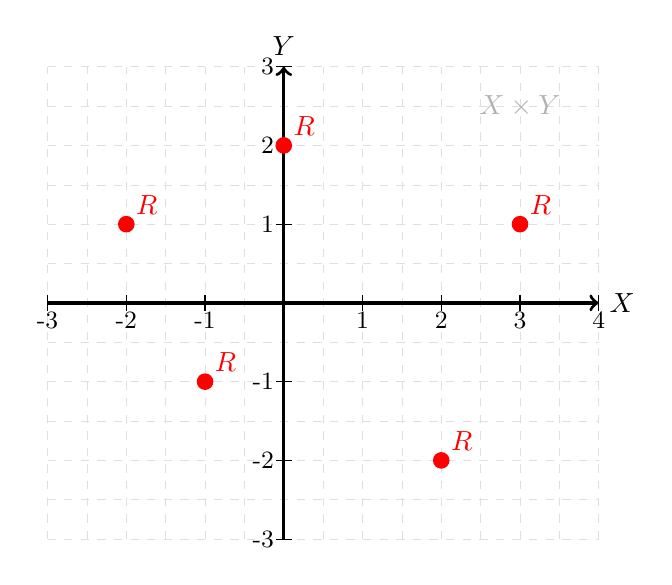
\begin{tikzpicture}
\draw[step=0.5cm, gray!25, very thin, dashed]
(-3.0,-3.0) grid (4.0,3.0);
\draw[gray!40, thin];
(-3.5,-3.5) rectangle (4.5,4.0);
\node[gray!60] at (3.0,2.5) {$X\times Y$};
\draw[->, very thick] (-3,0) -- (4,0) node[right] {$X$};
\draw[->, very thick] (0,-3) -- (0,3) node[above] {$Y$};
\foreach \x in {-3,-2,-1,1,2,3,4}
{
    \draw (\x,0.1) -- (\x,-0.1);
    \node[below] at (\x,0) {\small \x};
}
\foreach \y in {-3,-2,-1,1,2,3}
{
    \draw (0.1,\y) -- (-0.1,\y);
    \node[left] at (0,\y) {\small \y};
}
\foreach \x/\y in {-2/1, -1/-1, 0/2, 2/-2, 3/1}
{
    \fill[red] (\x,\y) circle (3pt);
    \node[above right] at (\x,\y) {\color{red}$R$};
}
\end{tikzpicture}
\end{center}
\begin{remark}
W definicji relacji $R\subseteq X\times Y$ istnieje pewna subtelność, którą należy wyjaśnić. Pisząc $R\subseteq X\times Y$ mamy na myśli dowolną czyli każdą relację pomiędzy $X$ i $Y$. Również pełną. Jeśli weźmiemy relację pełną pomiędzy $X$ i $Y$ to wówczas weźmiemy relację $R=X\times Y$. To nie jest tak, że $X\times Y$ jest relacją pełną inną od $R$ a $R$ jest każdą relacją pomiędzy tymi zbiorami ale nie pełną. Zauważmy, że relacja pełna pomiędzy $X$ i $Y$ skoro jest sobie równa to również się w sobie zawiera. Zatem zapis $R\subseteq X\times Y$ zawiera wszystkie możliwości. Łącznie z możliwością $R=X\times Y$ i wówczas również jest $R\subseteq X\times Y$. Jednocześnie łatwo zauważyć, że relacja pełna pomiędzy $X$ i $Y$ jest tylko jedna.$\\$
Ale skoro $R$ jest dowolnym podzbiorem relacji $X\times Y$ to $R\in\mathcal{P}(X\times Y)$.
\end{remark}
\begin{definition}
Niech $R\subseteq X\times Y$. Wówczas dziedziną relacji $R$ nazywamy zbiór: $dom(R)=\{x\in X:\exists y\in Y:(x,y)\in R\}$.$\\$
Stąd w naturalny sposób możemy zdefiniować przynależność elementu do dziedziny relacji $R$:
$x\in dom(R)\Leftrightarrow \exists y((x,y)\in R)$.
Rzecz jasna z definicji dziedziny relacji $R$ wynika, że $dom(R)\subseteq X$.
\end{definition}
\begin{remark}
Zaprzeczenie przynależności elementu do dziedziny relacji $R\subseteq X\times Y$.$\\$
$\neg x\in dom(R)\Leftrightarrow x\notin dom(R)\Leftrightarrow\not\exists y((x,y)\in R)\Leftrightarrow\forall y((x,y)\notin R)$.
Zatem $x\notin dom(R)\Leftrightarrow\forall y((x,y)\notin R)$.$\\$
{\scriptsize
\textbf{*Celowo pominąłem powyżej zapis $y\in Y$, bo $y\in Y$ wynika wprost z tego, że $R\subseteq X\times Y$}}
\end{remark}
\begin{definition}
Niech $R\subseteq X\times Y$. Wówczas zbiorem wartości relacji $R$ nazywamy zbiór: $rng(R)=\{y\in Y: \exists x\in X:(x,y)\in R\}$.
Stąd definiujemy przynależność elementu do zbioru wartości relacji $R$ jako: $y\in rng(R)\Leftrightarrow\exists x((x,y)\in R)$.
Łatwo zauważyć, że z definicji zbioru wartości relacji $R$ wynika, że $rng(R)\subseteq Y$.
\end{definition}
\begin{remark}
Zaprzeczenie przynależności elementu do zbioru wartości relacji $R\subseteq X\times Y$.$\\$
$\neg y\in rng(R)\Leftrightarrow y\notin rng(R)\Leftrightarrow\not\exists x((x,y)\in R)\Leftrightarrow\forall x((x,y)\notin R)$.
Zatem $y\notin rng(R)\Leftrightarrow\forall x((x,y)\notin R)$.$\\$
{
    \scriptsize
\textbf{*Powyżej celowo pominąłem $x\in X$, ponieważ $x\in X$ wprost wynika z tego, że $R\subseteq X\times Y$}
}
\end{remark}
\begin{property}
Niech $R\subseteq X\times Y$. W ogólności nie zachodzi: $R=dom(R)\times rng(R)$.
\end{property}
\begin{proof}[\textbf{Dowód}]
Ustalmy dowolną relację $R\subseteq X\times Y$. Niech $(x,y)\in R$. Wówczas z definicji iloczynu kartezjańskiego zbiorów wynika, że $x\in dom(R)$ i $y\in rng(R)$. Stąd $(x,y)\in dom(R)\times rng(R)$. Zatem otrzymujemy, że $(x,y)\in R\Rightarrow(x,y)\in dom(R)\times rng(R)$ co z definicji inkluzji relacji daje nam $R\subseteq dom(R)\times rng(R)$.$\\$
Niech $R=\{(x_{1},y_{1}),(x_{2},y_{2})\}$ oraz $R\subseteq X\times Y$, przy czym $x_{1}\ne x_{2}$ i $y_{1}\ne y_{2}$. Stąd $dom(R)=\{x_{1},x_{2}\}$ i $rng(R)=\{y_{1},y_{2}\}$. Wówczas $dom(R)\times rng(R)=\{(x_{1},y_{1}),(x_{1},y_{2}),(x_{2},y_{1}),(x_{2},y_{2})\}$. Zatem do relacji $R$ należą tylko dwie pary uporządkowane, które należą do zbioru $dom(R)\times rng(R)$ i żadne inne. Są to dokładnie pary $(x_{1},y_{1})$ i $(x_{2},y_{2})$. Stąd $dom(R)\times rng(R)\not\subseteq R$. $\\$
Ponieważ zachodzi tylko jedna inkluzja to zadana równość jest w ogólności fałszywa.
Jak widać z powyższej własności wprost wynika przynależność pary elementów $(x,y)$ do relacji $R$. Wówczas $(x,y)\in R\Rightarrow(x,y)\in dom(R)\times rng(R)$. Jak pokazał dowód, implikacja przeciwna w ogólności nie zachodzi.
\end{proof}
\begin{remark}
Innymi słowy: jeżeli element $x$ należy do dziedziny relacji $R$ i element $y$ należy do zbioru wartości tej relacji to nie oznacza to, że konkretna para uporządkowana $(x,y)$ należy do relacji $R$. Wówczas wiadomo natomiast, że jeżeli $x\in dom(R)$ to musi istnieć jakiś element $y$ ze zbioru $Y$, powiedzmy element $y'$ taki, że para uporządkowana $(x,y')$ należy do relacji $R$. Czyli z tego, że para uporządkowana $(x,y)$ należy do relacji $dom(R)\times rng(R)$ nie wynika, że ta konkretna para należy do relacji $R$. Wiadomo natomiast, że element $x$ z tej pary należy do jakiejś innej pary uporządkowanej, która należy do relacji $R$. I podobnie jest z elementem $y$ z tej pary. Para uporządkowana $(x,y)$ nie musi należeć do relacji $R$, ale jakaś para $(a,y)$ należy do relacji $R$. Wówczas wiadomo, że element $a$ jest elementem dziedziny relacji $R$.$\\$
Zatem podsumowując, z tego, że para uporządkowana $(x,y)$ należy do relacji $dom(R)\times rng(R)$ nie wynika, że ta para należy do relacji $R$ ale z tego wynika, że na pewno jakaś para uporządkowana, nazwijmy ją $(x,y')$- należy do relacji $R$ i jakaś para uporządkowana $(x',y)$ także należy do relacji $R$. Czyli jeżeli jakiś element należy do dziedziny relacji $R$ to z pewnością jest on argumentem w jakiejś parze uporządkowanej należącej do relacji $R$ ale niekoniecznie w relacji $R$ wartością tego argumentu jest ta sama wartość co wartość dla tego argumentu w relacji $dom(R)\times rng(R)$. I analogicznie dla elementu należącego do zbioru wartości relacji $R$. Z pewnością należy on do pewnej pary uporządkowanej z relacji $R$ ale niekoniecznie argumentem dla tej wartości w relacji $R$ będzie ten sam argument co w relacji $dom(R)\times rng(R)$. Można to zapisać jako: $(x,y)\in dom(R)\times rng(R)\Rightarrow\exists y'\in rng(R):(x,y')\in R\wedge\exists x'\in dom(R):(x',y)\in R$.
\end{remark}
\begin{remark}
M.in. w powyższym dowodzie nie mogliśmy ustalić dowolnych elementów $x$ i $y$, ponieważ nie każda para uporządkowana $(x,y)\in X\times Y$ należy do relacji $R$.
\end{remark}
\begin{property}
Niech $R\subseteq X\times Y$. W ogólności zachodzi: $R\subseteq dom(R)\times rng(R)$.
\end{property}
\begin{proof}[\textbf{Dowód}]
Dowód własności przedstawiony powyżej.
\end{proof}
\begin{definition}
Niech $X_{2}\subseteq X$ oraz $R\subseteq X\times Y$.
Wówczas relację $R\upharpoonright X_{2}=$ $=R\cap \left (X_{2}\times Y \right)=\{\left (x,y \right)\in R: x\in X_{2}\}$ nazywamy obcięciem relacji $R$ do zbioru $X_{2}$.
\end{definition}
\begin{remark}
Wprost z definicji relacji wynika, że obcięcie relacji $R$ do zbioru $X_{2}$ może być puste. W szczególności, gdy relacja $R$ jest pusta(czyli nie zawiera żadnych par uporządkowanych). Relacja $R$ nie zawiera żadnych par uporządkowanych wtedy i tylko wtedy, gdy jej dziedzina jest pusta lub gdy jej zbiór wartości(bądź przeciwdziedzina) jest pusty lub gdy zarówno jej dziedzina i zbiór wartości(bądź przeciwdziedzina) są zbiorami pustymi. Należy zauważyć, że ponieważ $rng(R)\subseteq Y$ to z tego wynika, że jeżeli $rng(R)=\emptyset$ to niekoniecznie przeciwdziedzina relacji $R$ jest pusta. Natomiast, gdy $Y=\emptyset$, czyli przeciwdziedzina relacji $R$ jest pusta to rzecz jasna $rng(R)=\emptyset$. Gdy jednak $R$ jest niepusta to jej obcięcie do zbioru $X_{2}$ będzie zbiorem pustym wtedy i tylko wtedy, gdy dziedzina obcięcia będzie pusta-wtedy i tylko wtedy, gdy zbiór $dom(R)\cap X_{2}$ będzie zbiorem pustym, a więc wtedy, gdy dziedzina relacji $R$ i dziedzina relacji $X_{2}\times Y$ będą zbiorami rozłącznymi(nie będą zawierały żadnych wspólnych elementów). Wówczas mimo, iż $rng(R)$ nie będzie zbiorem pustym(bo R jest niepuste) to wystarczy aby zbiór $dom(R)\cap X_{2}$ był pusty. Innymi słowy warunkiem koniecznym i wystarczającym dla niepustego obcięcia relacji do danego zbioru jest istnienie wspólnej części dziedziny tej relacji i zbioru do którego wykonywane jest obcięcie.
Należy też dodać, że z definicji relacji wynika, że relacja obcięcia relacji $R$ do zbioru $X_{2}$ może posiadać argumenty pochodzące ze zbiory $X_{2}$, a więc z jednego podzbioru zbioru $X$. Zauważmy też, że relacja $X_{2}\times Y$ jest
iloczynem kartezjańskim jednego podzbioru zbioru $X$ ze zbiorem $Y$. Mimo to, relacji obcięcia często nie da się przedstawić w układzie współrzędnych $OXY$
jako regularnie rozłożonych na płaszczyźnie par uporządkowanych. Oczywiście w pewnych przypadkach może być tak, że pary uporządkowane, których argumenty należą do par uporządkowanych z relacji $R$
które są też argumentami relacji $X_{2}\times Y$ tworzą na płaszczyźnie regularny prostokąt. Podkreślić jednak należy, że są to przypadki szczególne. Bowiem może być też
tak, że nie wszystkie argumenty pochodzące z par uporządkowanych relacji $R$, które są także argumentami par uporządkowanych relacji $X_{2}\times Y$
tworzą wszystkie możliwe pary uporządkowane z elementami ze zbioru wartości relacji $R$. Wówczas pary takie należą do relacji $X_{2}\times Y$ ale nie należą
wówczas do relacji $R$.
\end{remark}
\begin{definition}
Niech $X_{2}\subseteq X$ oraz $R\subseteq X\times Y$.
Wówczas dziedziną relacji $R\upharpoonright X_{2}=R\cap(X_{2}\times Y)$ jest zbiór $dom(R\upharpoonright X_{2})=dom(R)\cap X_{2}=\{x\in X_{2}: \exists y\in Y:(x,y)\in R\}$.$\\$
Możemy zatem zdefiniować przynależność elementu do dziedziny relacji $R\upharpoonright X_{2}$ jako
$x\in dom(R\upharpoonright X_{2})\Leftrightarrow x\in X_{2}\cap dom(R)\Leftrightarrow x\in X_{2}\wedge x\in dom(R)\Leftrightarrow x\in X_{2}\wedge\exists y((x,y)\in R)$.
\end{definition}
\begin{remark}
Zaprzeczenie przynależności elementu do dziedziny relacji $R\upharpoonright X_{2}$.
$\neg x\in dom(R\upharpoonright X_{2})\Leftrightarrow\neg x\in X_{2}\cap dom(R)\Leftrightarrow\neg(x\in X_{2}\wedge x\in dom(R))\Leftrightarrow\neg x\in X_{2}\vee\neg x\in dom(R)\Leftrightarrow (x\notin X_{2}\vee x\notin dom(R))\Leftrightarrow x\notin X_{2}\vee\forall y((x,y)\notin R)$
\end{remark}
\begin{definition}
Definicja przynależności pary elementów do relacji $R\upharpoonright X_{2}$.
Niech $X_{2}\subseteq X$ oraz $R\subseteq X\times Y$.
Niech $(x,y)\in R\upharpoonright X_{2}$. Wówczas z definicji obcięcia relacji $R$ do zbioru $X_{2}$ wynika, że $(x,y)\in R\cap(X_{2}\times Y)$. Zatem z definicji przekroju zbiorów otrzymujemy $(x,y)\in R$ i $(x,y)\in X_{2}\times Y$. Stąd z definicji iloczynu kartezjańskiego zbiorów jest $x\in X_{2}$ i $y\in Y$. Wówczas mamy $(x,y)\in R$ i $x\in X_{2}$ i $y\in Y$. Ponieważ $rng(R)\subseteq Y$ to możemy pominąć $y\in Y$ i dostajemy $(x,y)\in R$ i $x\in X_{2}$. Zatem z definicji dziedziny relacji wynika, że $x\in dom(R)$, zaś z definicji zbioru wartości relacji jest $y\in rng(R)$. Czyli otrzymujemy $x\in dom(R)$ i $y\in rng(R)$ i $x\in X_{2}$. Korzystając z przemienności i łączności koniunkcji otrzymujemy zatem $(x\in dom(R)$ i $x\in X_{2})$ i $y\in rng(R)$. Wówczas z definicji przekroju zbiorów jest $x\in dom(R)\cap X_{2}$ i $y\in rng(R)$ co z definicji iloczynu kartezjańskiego zbiorów daje nam $(x,y)\in(dom(R)\cap X_{2})\times rng(R)$. Korzystając z prawostronnej rozdzielności iloczynu kartezjańskiego względem przekroju zbiorów możemy zapisać $(x,y)\in(dom(R)\times rng(R))\cap(X_{2}\times rng(R))$. Wówczas otrzymujemy, że $R\upharpoonright X_{2}\subseteq(dom(R)\cap X_{2})\times rng(R)$. Jest to jedna z własności obcięcia relacji $R$ do zbioru $X_{2}$.
\end{definition}
\begin{definition}
Z definicji przynależności pary elementów do relacji $R\upharpoonright X_{2}$ możemy wprost wyprowadzić definicję
zbioru wartości tejże relacji. Mianowicie:
niech $X_{2}\subseteq X$ oraz $R\subseteq X\times Y$. Zbiorem wartości relacji $R\upharpoonright X_{2}=R\cap(X_{2}\times Y)$ jest zbiór $rng(R\upharpoonright X_{2})=rng(R\cap(X_{2}\times Y))=\{y\in rng(R):\exists x\in dom(R)\cap X_{2}:(x,y)\in R\}$.  Jest to równoważne zapisowi:
$\\$ $rng(R\upharpoonright X_{2})=rng(R\cap(X_{2}\times Y))=\{y\in Y:\exists x\in X_{2}:(x,y)\in R\}$.
\end{definition}
\begin{remark}
Zaprzeczenie definicji przynależności elementu do zbioru wartości relacji $R\upharpoonright X_{2}$.$\\$
$\neg y\in rng(R\upharpoonright X_{2})\Leftrightarrow\neg y\in rng(R\cap(X_{2}\times Y))\Leftrightarrow y\notin rng(R\upharpoonright X_{2})\Leftrightarrow y\notin rng(R\cap(X_{2}\times Y))\Leftrightarrow\neg\exists x\in dom(R)\cap X_{2}((x,y)\in R)\Leftrightarrow\not\exists x\in dom(R)\cap X_{2}((x,y)\in R)\Leftrightarrow\forall x\in dom(R)\cap X_{2}((x,y)\notin R)$.
\end{remark}
\begin{remark}
Zaprzeczenie definicji przynależności pary uporządkowanej do relacji $R\upharpoonright X_{2}$.
Niech $X_{2}\subseteq X$ oraz $R\subseteq X\times Y$. Wówczas z definicji obcięcia relacji $R$ do zbioru $X_{2}$ wynika, że $(x,y)\notin R\upharpoonright X_{2}\Leftrightarrow(x,y)\notin R\cap(X_{2}\times Y)$. Stąd z definicji przekroju zbiorów otrzymujemy $(x,y)\notin R$ lub $(x,y)\notin X_{2}\times Y$. Zatem z definicji iloczynu kartezjańskiego zbiorów mamy $(x,y)\notin R$ lub $x\notin X_{2}$ lub $y\notin Y$. Ale z założenia $x\in X$ i $y\in Y$ czyli warunek $y\notin Y$ jest fałyszywy. Stąd otrzymujemy, że $(x,y)\notin R\upharpoonright X_{2}\Leftrightarrow(x,y)\notin R$ lub $x\notin X_{2}$. Jest to równoważne temu, że $\forall(x,y)\in X\times Y:(x,y)\notin R\upharpoonright X_{2}\Leftrightarrow(x,y)\notin R\vee x\notin X_{2}$.
\end{remark}
\begin{property}
Niech $X_{2}\subseteq X$ i $R\subseteq X\times Y$. W ogólności nie zachodzi równość: $R\upharpoonright X_{2}=(dom(R)\cap X_{2})\times rng(R)$.
\end{property}
\begin{proof}[\textbf{Dowód}]
Niech $R=\{(x_{1},y_{1}),(x_{2},y_{2})\}$, $X_{2}=\{x_{1},x_{2}\}$. Przy czym rozważane elementy są parami różne. Wówczas $dom(R)=\{x_{1},x_{2}\}$ oraz $rng(R)=\\=\{y_{1},y_{2}\}$. Stąd $dom(R)\cap X_{2}=\{x_{1},x_{2}\}$. Zatem $(dom(R)\cap X_{2})\times rng(R)=\\=\{(x_{1},y_{1}),(x_{1},y_{2}),(x_{2},y_{1}),(x_{2},y_{2})\}$. Łatwo wówczas zauważyć, że $(x_{1},y_{2})\notin R$ i $(x_{2},y_{1})\notin R$. A zatem $(x_{1},y_{2})\notin R\upharpoonright X_{2}$ i $(x_{2},y_{1})\notin R\upharpoonright X_{2}$. Stąd w ogólności nie zachodzi inkluzja $[(dom(R)\cap X_{2})\times rng(R)]\subseteq R\upharpoonright X_{2}$. Wówczas zadana równość nie zachodzi w ogólności.
\end{proof}
\begin{property}
Dla dowolnego zbioru $X_{2}\subseteq X$ oraz dla dowolnej relacji $R\subseteq X\times Y$ zachodzi $R\upharpoonright X_{2}\ne\emptyset\Rightarrow dom(R)\cap X_{2}\ne\emptyset$.
\end{property}
\begin{proof}[\textbf{Dowód}]
Ustalmy dowolny zbiór $X_{2}\subseteq X$ oraz dowolną relację $R\subseteq X\times Y$. Niech $R\upharpoonright X_{2}\ne\emptyset$. Wówczas z definicji obcięcia relacji $R$ do zbioru $X_{2}$ wynika, że $R\cap(X_{2}\times Y)\ne\emptyset$. Niech $(x,y)\in R\upharpoonright X_{2}$. Stąd $(x,y)\in R\cap(X_{2}\times Y)$. Zatem z definicji przekroju relacji otrzymujemy, że $(x,y)\in R$ i $(x,y)\in X_{2}\times Y$. Stąd z definicji relacji wynika, że istnieje takie $y\in rng(R)$  dla którego $(x,y)\in R$, a następnie z definicji dziedziny relacji jest $x\in dom(R)$ i $y\in rng(R)$ i $x\in X_{2}$ i $y\in Y$. Pomijając przynależność elementu $y$ do zbioru $rng(R)$ i do zbioru $Y$ mamy $x\in dom(R)$ i $x\in X_{2}$ co z definicji przekroju zbiorów daje nam $x\in dom(R)\cap X_{2}$. Wówczas skoro z przynależności pary uporządkowanej $(x,y)$ do relacji $R\upharpoonright X_{2}$ wynika przynależność elementu $x$ do zbioru $dom(R)\cap X_{2}$ to zachodzi zadana implikacja. Bowiem z przynależności pary uporządkowanej do relacji $R\upharpoonright X_{2}$ wynika, że relacja ta jest niepusta. Wówczas jeśli jest niepusta to iloczyn $dom(R)\cap X_{2}$ także jest niepusty, ponieważ należy do niego element $x$.
\end{proof}
\begin{remark}
W powyższym dowodzie nie ustalaliśmy dowolnych elementów $x$ i $y$, ponieważ byłoby to założenie błędne. Bowiem nie każda para uporządkowana $(x,y)\in X\times Y$, należy do relacji $R$, bądź nie każdy
element $x\in X_{2}$. Pisząc, "niech $(x,y)\in R\upharpoonright X_{2}$" nie ustalamy dowolnych $x,y$. Jest to po prostu pewna para uporządkowana należąca do relacji $R$, której należenie do tej relacji zapewnia założenie $R\upharpoonright X_{2}\ne\emptyset$.
\end{remark}
\begin{property}
Dla dowolnego zbioru $X_{2}\subseteq X$ oraz dla dowolnej relacji $R\subseteq X\times Y$ zachodzi $dom(R)\cap X_{2}\ne\emptyset\Rightarrow R\upharpoonright X_{2}\ne\emptyset$.
\end{property}
\begin{proof}[\textbf{Dowód}]
Ustalmy dowolny zbiór $X_{2}\subseteq X$ oraz dowolną relację $R\subseteq X\times Y$. Niech $dom(R)\cap X_{2}\ne\emptyset$. Weźmy dowolny element $x\in dom(R)\cap X_{2}$. Wówczas z definicji przekroju zbiorów wynika, że $x\in dom(R)$ i $x\in X_{2}$. Z definicji przynależności elementu $x$ do dziedziny relacji $R$ otrzymujemy, że istnieje $y\in Y$ dla którego $(x,y)\in R$. Ale skoro $x\in X_{2}$ to $(x,y)\in X_{2}\times Y$, bo z definicji iloczynu kartezjańskiego zbiorów wynika, że relacja $X_{2}\times Y$ zawiera wszystkie pary uporządkowane $(x,y)$ przy spełnionym warunku $x\in X_{2}$. Stąd dostajemy $(x,y)\in R$ i $(x,y)\in X_{2}\times Y$. Zatem z definicji przekroju relacji jest $(x,y)\in R\cap(X_{2}\times Y)$. Co z definicji obcięcia relacji $R$ do zbioru $X_{2}$ daje nam $(x,y)\in R\upharpoonright X_{2}$. Wówczas z niepustości zbioru $dom(R)\cap X_{2}$ wynika niepustość relacji $R\upharpoonright X_{2}$. Stąd w ogólności zachodzi zadana implikacja.$\\$
Ale skoro zachodzą obie przeciwne implikacje to w ogólności zachodzi równoważność $R\upharpoonright X_{2}\ne\emptyset\Leftrightarrow dom(R)\cap X_{2}\ne\emptyset$.
Co naturalnie prowadzi nas do równoważności $R\upharpoonright X_{2}=\emptyset\Leftrightarrow dom(R)\cap X_{2}=\emptyset$.
\end{proof}
\begin{remark}
Rzecz godna uwagi odnośnie udowodnionej równoważności $R\upharpoonright X_{2}\ne\emptyset\Leftrightarrow dom(R)\cap X_{2}\ne\emptyset$ jest taka, że wystarczy aby dziedzina relacji $R$ i zbiór $X_{2}$ miały choćby jeden element wspólny i wówczas obcięcie relacji $R$ do zbioru $X_{2}$ jest niepuste. To jednak zachodzi w tak-można powiedzieć-prosty sposób ze względu na "prostokątność" relacji $X_{2}\times Y$. "Prostokątność" czyli to, że dana relacja daje się w geometryczny sposób zinterpretować na płaszczyźnie $OXY$ jako regularny prostokąt. Co nam to daje? W tym wypadku wiemy, że każdy element $y$ ze zbioru $Y$ jest w parze z argumentem ze zbioru $X_{2}$. Wówczas jeśli dziedzina relacji $R$ i zbiór $X_{2}$ mają wspólny element to nie musimy sprawdzać czy dana para uporządkowana z relacji $R$ zawierająca wspólny argument należy też do relacji $X_{2}\times Y$. Bowiem wiadomo, że wspólny argument łączy się z każdym $y$ w relacji $X_{2}\times Y$ i jakaś para takiego wspólnego argumentu z pewnym $y$ należy i do relacji $X_{2}\times Y$ i do relacji $R$ ze względu na wspólny argument. To właśnie ułatwia "prostokątność" relacji $X_{2}\times Y$. Wiemy oczywiście, że taka wspólna para uporządkowana może być jedna dla relacji $R$ i $X_{2}\times Y$, ponieważ relacja $R$ na ogół nie jest "prostokątna". Ale "prostokątność" relacji $X_{2}\times Y$ znacznie upraszcza niepustość obcięcia relacji $R$ do zbioru $X_{2}$. Zatem zadana równoważność zachodzi w gruncie rzeczy ze  względu na argument z par uporządkowanych a nie na argument i jego wartość. I to właśnie daje "prostokątność" relacji $X_{2}\times Y$. A z kolei "prostokątność" relacji $X_{2}\times Y$ wynika wprost z tego, że jest to relacja pełna pomiędzy $X_{2}$ i $Y$. Tak więc finalizując można powiedzieć, że o niepustości relacji obcięcia decyduje wspólny argument dla relacji $R$ i relacji $X_{2}\times Y$ oraz to, że relacja pomiędzy $X_{2}$ i $Y$ jest relacją pełną. A z tego, że jest to relacja pełna wynika jej "prostokątność".
"Prostokątność" relacji jest bowiem interpretacją geometryczną pełności relacji.$\\$
Chciałbym też podkreślić, że pisząc o "prostokątności" relacji mam na myśli niekoniecznie to, że pary uporządkowane danej relacji tworzą w układzie
współrzędnych wyraźny prostokąt. Może to być np. linia prostopadła do osi $OX$. Chodzi o to aby dana relacja zawierała wszystkie możliwe pary uporządkowane jakie
da się w niej utworzyć. W przypadku relacji $X_{2}\times Y$ będą to wszystkie możliwe pary uporządkowane $(x,y)$, gdzie $x\in X_{2}$. Wówczas pojęcie "prostokątności"
dotyczy relacji $X_{2}\times Y$.
\end{remark}
\begin{definition}
Niech $R\subseteq X\times Y$ i $S\subseteq Y\times W$. Relację $S\circ R=\{(x,w)\in X\times W:\exists y\in Y:(x,y)\in R\wedge(y,w)\in S\}$ nazywamy złożeniem relacji $R$ i $S$.$\\$
Z definicji złożenia relacji wynika, że $rng(R)\subseteq Y$ i $dom(S)\subseteq Y$. Ale skoro istnieje $y\in Y$ dla którego $(x,y)\in R$ i $(y,w)\in S$ to istnieje $y\in rng(R)\cap dom(S)$ dla którego $(x,y)\in R$ i $(y,w)\in S$. Wówczas definicja złożenia relacji przyjmuje postać $S\circ R=\{(x,w)\in X\times W:\exists y\in rng(R)\cap dom(S): (x,y)\in R\wedge(y,w)\in S\}$.
Jednakże z tego, że $(x,y)\in R$ wynika, że $y\in rng(R)$, zaś z $(y,w)\in S$ wynika $y\in dom(S)$.
Stąd ostatni sposób zapisania definicji złożenia relacji aczkolwiek poprawny logicznie zawiera reduntatne warunki. Dlatego bardziej formalny jest zapis pierwszy.
\end{definition}
\begin{remark}
Zauważmy, że złożenia relacji także nie daje się w ogólności przedstawić geometrycznie w układzie współrzędnych $0XY$ jako zbioru par uporządkowanych tworzących prostokąt. Ale z innego względu niż było to w przypadku relacji $R\subseteq X\times Y$ czy obcięcia relacji $R\upharpoonright X_{2}$. Otóż ogólna niemożność przedstawienia na płaszczyźnie złożenia relacji nie wynika bezpośrednio z tego, że relacje, które składamy na ogół nie dają się przedstawić w układzie współrzędnych jako prostokąty. Składając relacje $R\subseteq X\times Y$ i $S\subseteq Y\times W$ musi być spełniony warunek konieczny i wystarczający aby istniał taki element ze zbioru $rng(R)\cap dom(S)$ dla którego $(x,y)\in R$ i $(y,w)\in S$. Wówczas para uporządkowana $(x,w)$ należy do złożenia $S\circ R$. Tak więc jeśli nawet relacje $R$ i $S$ nie dają się zinterpretować geometrycznie jako prostokąty to jeśli istnieje wspomniany element $y$ wspólny dla par uporządkowanych z relacji $R$ i relacji $S$, mianowicie taki, że w parze elementów należących do relacji $R$ jest on wartością dla danego argumentu, zaś w parze elementów należących do relacji $S$ jest argumentem- to jego istnienie i powiązanie go z konkretnymi elementami $x$ w relacji $R$ i  $w$ w relacji $S$ powoduje takie a nie inne rozmieszczenie par $(x,y)$ i $(y,w)$ w układzie współrzędnych, które na ogół nie jest regularne. Tak więc z samej interpretacji geometrycznej relacji składanych nie wynika wprost interpretacja geometryczna ich złożenia. Kluczowym jest tutaj element   $y$ wspólny dla par uporządkowanych z obu relacji.$\\$
Należy zatem zdawać sobie sprawę z tego, że złożenie relacji $S\circ R$ nie jest  pełną relacją $X\times W$. Jest to relacja $S\circ R\subseteq X\times W$ ale z określonym warunkiem istnienia elementu "łączącego" elementy z $X$ z elementami z $W$.
\end{remark}
\begin{property}
Niech $R\subseteq X\times Y$ i $S\subseteq Y\times W$. Wówczas zachodzi równoważność $S\circ R\ne\emptyset\Leftrightarrow dom(S)\cap rng(R)\ne\emptyset$.
\end{property}
\begin{proof}[\textbf{Dowód}]
Ustalmy dowolne relacje $R\subseteq X\times Y$ i $S\subseteq Y\times W$. Niech $S\circ R\ne\emptyset$ i $(x,w)\in S\circ R$. Wówczas z definicji złożenia relacji wynika, że istnieje $y\in Y$ dla którego $(x,y)\in R$ i $(y,w)\in S$. Stąd $y\in rng(R)$ i $y\in dom(S)$ co z definicji przekroju zbiorów daje nam $y\in rng(R)\cap dom(S)$. Wówczas $rng(R)\cap dom(S)\ne\emptyset$. Zatem prawdziwa jest implikacja
 $S\circ R\ne\emptyset\Rightarrow dom(S)\cap rng(R)\ne\emptyset$.$\\$
Ustalmy dowolne relacje $R\subseteq X\times Y$ i $S\subseteq Y\times W$. Niech $rng(R)\cap dom(S)\ne\emptyset$ i $y\in rng(R)\cap dom(S)$. Wówczas z definicji przekroju zbiorów wynika, że $y\in rng(R)$ i $y\in dom(S)$. Stąd z definicji przynależności elementu do zbioru wartości relacji $R$ otrzymujemy, że istnieje taki element $x\in X$ dla którego $(x,y)\in R$, zaś z definicji przynależności elementu do dziedziny relacji $S$ dostajemy, że istnieje taki element $w\in W$ dla którego $(y,w)\in S$. Wówczas skoro $y$ jest elementem wspólnym dla par uporządkowanych $(x,y)\in R$ i $(y,w)\in S$ to z definicji złożenia relacji wynika, że $(x,w)\in S\circ R$. Zatem $S\circ R\ne\emptyset$. Stąd zachodzi implikacja $rng(R)\cap dom(S)\ne\emptyset\Rightarrow S\circ R\ne\emptyset$.$\\$
Ponieważ zachodzą obie implikacje to zadana równoważność jest w ogólności prawdziwa.
\end{proof}
\begin{definition}
Niech $R\subseteq X\times Y$ i $S\subseteq Y\times W$. Wówczas
zbiór $dom(S\circ R)=$ $=\{x\in X:\exists y\in rng(R)\cap dom(S):(x,y)\in R\}$ nazywamy dziedziną złożenia relacji $S\circ R$. Równoważnie $dom(S\circ R)=\{x\in X:\exists y\in dom(S):(x,y)\in R\}$
Zauważmy, że skoro $y\in rng(R)$ to istnieje $x\in X$ takie, że $(x,y)\in R$. To wówczas jeżeli jeszcze ten sam $y\in dom(S)$ to z definicji istnieje taki $w\in W$, że $(y,w)\in S$. A zatem $(x,w)\in S\circ R$.
Tak więc warunek $y\in rng(R)$ jest w tym wypadku redundantny, bo skoro $(x,y)\in R$ to $y\in rng(R)$.
$\\$ Możemy zatem określić przynależność elementu do dziedziny złożenia. Mianowicie $x\in dom(S\circ R)\Leftrightarrow\exists y\in dom(S):(x,y)\in R$
bądź $x\in dom(S\circ R)\Leftrightarrow\exists w\in W:(x,w)\in S\circ R$. Oba zapisy są równoważne.
\end{definition}
\begin{remark}
Zaprzeczenie przynależności elementu do dziedziny złożenia relacji $S\circ R$.$\\$
$\neg x\in dom(S\circ R)\Leftrightarrow x\notin dom(S\circ R)\Leftrightarrow\neg(\exists y\in dom(S):(x,y)\in R)\Leftrightarrow\forall y\in dom(S):(x,y)\notin R$.
\end{remark}
\begin{definition}
Niech $R\subseteq X\times Y$ i $S\subseteq Y\times W$. Wówczas
zbiór $rng(S\circ R)=$ $=\{w\in W:\exists y\in rng(R)\cap dom(S):(y,w)\in S\}$ nazywamy zbiorem wartości relacji $S\circ R$.$\\$
W tym przypadku niepotrzebne jest podawanie warunku $y\in dom(S)$, ponieważ wynika on z tego, że $(y,w)\in S$. Zatem warunek $y\in dom(S)$ jest w tym wypadku renduntantny i wystarczy sam warunek $y\in rng(R)$. Wówczas $rng(S\circ R)=\{w\in W:\exists y\in rng(R):(y,w)\in S\}$.
W naturalny sposób możemy stąd zdefiniować przynależność elementu do zbioru wartości relacji złożenia $S\circ R$. Zatem $w\in rng(S\circ R)\Leftrightarrow\exists y\in rng(R):(y,w)\in S$.
Bądź $w\in rng(S\circ R)\Leftrightarrow\exists x\in X:(x,w)\in S\circ R$. Oba zapisy są równoważne.
\end{definition}
\begin{remark}
Zaprzeczenie przynależności elementu do zbioru wartości złożenia relacji $S\circ R$.$\\$
$\neg w\in rng(S\circ R)\Leftrightarrow w\notin rng(S\circ R)\Leftrightarrow\neg(\exists y\in Y:(y,w)\in S\wedge y\in rng(R))\Leftrightarrow\forall y\in Y:(y,w)\notin S\vee y\notin rng(R)$.
Badź $w\notin rng(S\circ R)\Leftrightarrow\neg(\exists y\in rng(R):(y,w)\in S)\Leftrightarrow\forall y\in rng(R):(y,w)\notin S$.
\end{remark}
\begin{property}
Zauważmy, że z definicji dziedziny złożenia $S\circ R$ wynika wprost zależność $dom(S\circ R)\subseteq dom(R)$. Bowiem istnienie elementu $y\in rng(R)\cap dom(S)$ dla którego $(x,y)\in R$ oznacza, że $x\in dom(S\circ R)$. I przeciwnie.  Ale skoro $(x,y)\in R$ to $x\in dom(R)$. Należy podkreślić wówczas, że nie każdy element $x$ należący do pary uporządkowanej $(x,y)\in R$ może należeć do dziedziny złożenia $S\circ R$. Tylko te elementy $x$ z par $(x,y)\in R$ będą należeć do dziedziny złożenia $S\circ R$, których wartości będą należeć do dziedziny relacji $S$. A zatem $dom(S\circ R)\subseteq dom(R)$.$\\$
Z tego łatwo wywnioskować, że inkluzja przeciwna w ogólności nie zachodzi. Bowiem jeśli nie każdy element $x$ z par uporządkowanych $(x,y)$ należących do relacji $R$ ma wartość $y$, należącą do dziedziny relacji $S$ to wówczas dziedzina relacji $R$ zawiera elementy, które nie należą do dziedziny relacji złożenia $S\circ R$. Wówczas dziedzina relacji $R$ nie zawiera się w dziedzinie relacji złożenia. A skoro jedna z inkluzji nie zachodzi w ogólności to w ogólności nie zachodzi równość $dom(S\circ R)=dom(R)$.$\\$
Można to też ująć w bardziej szczegółowy sposób. Do relacji $R$ może należeć taka para uporządkowana $(x,y)$, z której
element $y$ nie należy do żadnej z par uporządkowanych $(y',w)$ z relacji $S$. Czyli $y\ne y'$. Wówczas rzecz jasna para uporządkowana
$(x,w)$ należy do relacji pełnej $X\times W$ ale nie należy do złożenia $S\circ R$. Zatem warunkiem koniecznym i wystarczającym należenia
pary uporządkowanej $(x,w)$ do złożenia relacji $S\circ R$ jest należenie pary uporządkowanej $(x,y)$ do relacji $R$ i pary uporządkowanej
$(y,w)$ do relacji $S$, gdzie oczywiście $y$ jest elementem wspólnym dla obu par. Innymi słowy: jeżeli $R(x)=y$ i $S(y)=w$
to para uporządkowana $(x,w)$ należy do złożenia $S\circ R$. I rzecz jasna przeciwnie: jeżeli $(x,w)$ należy do złożenia
relacji $S\circ R$ to $R(x)=y$ i $S(y)=w$.
\end{property}
\begin{definition}
Definicja przynależności pary uporządkowanej do złożenia relacji. Niech $R\subseteq X\times Y$ i $S\subseteq Y\times W$. Wówczas
$(x,w)\in S\circ R\Leftrightarrow[(x,y)\in dom(R)\times rng(R)\Leftrightarrow(x,y)\in dom(R)\times dom(S)]$ i $[(x,y)\in R$ i $(y,w)\in S]$.$\\$
Bardziej formalnie:
$(x,w)\in S\circ R\Leftrightarrow\exists y\in Y:(x,y)\in R\wedge(y,w)\in S$
\end{definition}
\begin{remark}
Zaprzeczenie przynależności pary uporządkowanej do złożenia relacji.$\\$
$\neg (x,w)\in S\circ R\Leftrightarrow(x,w)\notin S\circ R\Leftrightarrow\neg\exists y\in Y:(x,y)\in R\wedge(y,w)\in S\Leftrightarrow\forall y\in Y:(x,y)\notin R\vee(y,w)\notin S$.
\end{remark}
\begin{property}
Niech $R\subseteq X\times Y$ i $S\subseteq Y\times W$. Wówczas w ogólności zachodzi inkluzja $rng(S\circ R)\subseteq rng(S)$.
\end{property}
\begin{proof}[\textbf{Dowód}]
Ustalmy dowolne relacje $R\subseteq X\times Y$ i $S\subseteq Y\times W$. Niech $w\in rng(S\circ R)$. Wówczas z definicji zbioru wartości złożenia relacji wynika, że istnieje $y\in rng(R)\cap dom(S)$ dla którego $(y,w)\in S$. Ale wówczas $w\in rng(S)$. Zatem mamy $w\in rng(S\circ R)\Rightarrow w\in rng(S)$ co z definicji inkluzji zbiorów daje nam $rng(S\circ R)\subseteq rng(S)$.
\end{proof}
\begin{property}
Niech $S\subseteq Y\times W$ i $R\subseteq X\times Y$. W ogólności nie zachodzi równość $rng(S\circ R)=rng(S)$.
\end{property}
\begin{proof}[\textbf{Dowód}]
Niech $R=\{(x_{1},y_{1}),(x_{2},y_{2})\}$ i $S=\{(y_{1},w_{1}),(y_{3},w_{3})\}$. Przy czym rozważane elementy są parami różne. Wówczas z definicji złożenia relacji wynika, że $S\circ R=\{(x_{1},w_{1})\}$. Zatem $rng(S\circ R)=\{w_{1}\}$, zaś $rng(S)=\{w_{1},w_{3}\}$. Ale wówczas $rng(S\circ R)\ne rng(S)$.
Czyli zadana równość w ogólności nie zachodzi.
\end{proof}
\begin{exercise}
Z samego warunku istnienia elementu $y\in rng(R)\cap dom(S)$ nie wynika, że para uporządkowana $(x,y)\in R$, ponieważ z tego, że $y\in rng(R)$ nie wynika istnienie elementu $x\in X$ dla którego $(x,y)\in R$. Jeśli $x\in dom(R)$ i $y\in rng(R)$ to para uporządkowana $(x,y)\in dom(R)\times rng(R)$ ale niekoniecznie ta sama para uporządkowana należy do relacji $R$. Z pewnością jednak istnieje tak element $x'\in dom(R)$, że para $(x',y)\in R$. I podobnie skoro $y\in dom(S)$ to para uporządkowana $(y,w)\in dom(S)\times rng(S)$. Wówczas z tego nie wynika, że para $(y,w)\in S$ ale wiadomo wówczas, że istnieje taki element $w'\in rng(S)$, że para uporządkowana $(y,w')\in S$. Stąd na mocy definicji złożenia relacji $S\circ R$ otrzymujemy, że para uporządkowana $(x',w')\in S\circ R$. Zauważmy jednak, że $x'\in dom(S\circ R)$ i $w'\in rng(S\circ R)$. Stąd z definicji iloczynu kartezjańskiego zbiorów dostajemy, że $(x',w')\in dom(S\circ R)\times rng(S\circ R)$. Zatem skoro każda z par uporządkowanych $(x',w')\in S\circ R$ należy także do relacji $dom(S\circ R)\times rng(S\circ R)$ to z definicji inkluzji zbiorów jest $S\circ R\subseteq dom(S\circ R)\times rng(S\circ R)$.
\end{exercise}
\begin{property}
Niech $S\subseteq Y\times W$ i $R\subseteq X\times Y$. W ogólności nie zachodzi równość $S\circ R=dom(S\circ R)\times rng(S\circ R)$.
\end{property}
\begin{proof}[\textbf{Dowód}]
Niech $R=\{(x_{1},y_{1}),(x_{2},y_{2})\}$ i $S=\{(y_{1},w_{1}),(y_{2},w_{2})\}$. Przy czym rozważane elementy są parami różne. Wówczas z definicji wynika, że $S\circ R=\{(x_{1},w_{1}),(x_{2},w_{2})\}$. Stąd $dom(S\circ R)=\{x_{1},x_{2}\}$ oraz $rng(S\circ R)=\{w_{1},w_{2}\}$ ale $dom(S\circ R)\times rng(S\circ R)=\\=\{(x_{1},w_{1}),(x_{1},w_{2}),(x_{2},w_{1}),(x_{2},w_{2})\}$. Od razu widać, że pary uporządkowane $(x_{1},w_{2})$ i $(x_{2},w_{1})$ nie należą do relacji $S\circ R$. Zatem w ogólności zadana równość nie może zachodzić.
\end{proof}
\begin{remark}
Z powyższego dowodu można wyraźniej dostrzec naturę złożenia relacji. Intuicyjnie mogłoby się wydawać, iż dla złożenia relacji $S\circ R$ prawdziwa jest równość $S\circ R=dom(S\circ R)\times rng(S\circ R)$. Ale gdy głębiej przyjrzymy się strukturze złożenia relacji to zauważymy, że wszystko dzieje się na poziomie relacji $R$ i $S$. Co to oznacza? Na przykładzie powyższego dowodu widzimy, że elementy $x_{1}$ i $w_{1}$ mają wspólny element pośredni czyli element $y_{1}$. Dlatego, że $(x_{1},y_{1})\in R$ i $(y_{1},w_{1})\in S$. Stąd z definicji złożenia relacji jest $(x_{1},w_{1})\in S\circ R$. Podobnie jest z elementami $x_{2}$ i $w_{2}$ tyle, że ich elementem pośrednim w złożeniu $S\circ R$ jest $y_{2}$. Wówczas przykładowe złożenie $S\circ R$ nie wykorzystuje wszystkich możliwości. Bowiem $x_{1}$ nie tworzy pary uporządkowanej z $y_{2}$ w relacji $R$ i $x_{2}$ nie tworzy pary z $y_{1}$ w tejże relacji. Ale relacja $dom(S\circ R)\times rng(S\circ R)$ tworzy wszystkie możliwe pary uporządkowane elementów $x_{1}, x_{2}$ z elementami $w_{1}, w_{2}$ pomimo tego, iż element $x_{1}$ w złożeniu $S\circ R$ nie łączy się z elementem $w_{2}$ i element $x_{2}$ w tym złożeniu nie łączy się z elementem $w_{1}$. Jak widać relacja $dom(S\circ R)\times rng(S\circ R)$ działa jakoby na wyższym, szerszym poziomie niż złożenie $S\circ R$. W konsekwencji zachodzi zależność:
$S\circ R\subseteq dom(S\circ R)\times rng(S\circ R)\subseteq X\times W$.
\end{remark}
\begin{property}
Składanie relacji nie jest przemienne.
\end{property}
\begin{remark}
Z definicji złożenia relacji $S\circ R$ wynika wprost nieprzemienność składania relacji. Zauważmy, że o ile $S\circ R=\{(x,w)\in X\times W:\exists y\in Y:(x,y)\in R\wedge(y,w)\in S\}$ to $(R\circ S)$ może być złożeniem pustym jeśli zbiory $X$ i $W$ nie mają elementów wspólnych. Dlatego w ogólności $S\circ R\ne R\circ S$.
\end{remark}
\begin{property}
Składanie relacji jest łączne.
\end{property}
\begin{proof}[\textbf{Dowód}]
Niech $R\subseteq X\times Y,S\subseteq Y\times W$ i $T\subseteq W\times Z$. Weźmy $(x,z)\in T\circ(S\circ R)$. Wówczas z definicji złożenia relacji wynika, że istnieje $w\in W$ dla którego $(x,w)\in S\circ R$ i $(w,z)\in T$. Ponieważ $(x,w)\in S\circ R$ to z definicji złożenia relacji istnieje $y\in Y$ dla którego $(x,y)\in R$ i $(y,w)\in S$. Ale skoro $(y,w)\in S$ i $(w,z)\in T$ to z definicji złożenia relacji jest $(y,z)\in T\circ S$. Zatem z definicji istnieje $y\in Y$ dla którego $(x,y)\in R$ i $(y,z)\in T\circ S$, a wówczas $(x,z)\in(T\circ S)\circ R$. Ponieważ każda para uporządkowana ze złożenia relacji $T\circ(S\circ R)$ należy do złożenia $(T\circ S)\circ R$ to $T\circ(S\circ R)\subseteq(T\circ S)\circ R$.$\\$
Niech $R\subseteq X\times Y,S\subseteq Y\times W$ i $T\subseteq W\times Z$. Weźmy $(x,z)\in(T\circ S)\circ R$. Wówczas z definicji złożenia relacji wynika, że istnieje $y\in Y$ dla którego $(x,y)\in R$ i $(y,z)\in T\circ S$. Ponieważ $(y,z)\in T\circ S$ to z definicji złożenia relacji istnieje $w\in W$ dla którego $(y,w)\in S$ i $(w,z)\in T$. Ale istnieje $y\in Y$ dla którego $(x,y)\in R$ i $(y,w)\in S$ co z definicji złożenia relacji daje $(x,w)\in S\circ R$. Zatem istnieje $w\in W$ dla którego $(x,w)\in S\circ R$ i $(w,z)\in T$. Stąd $(x,z)\in T\circ(S\circ R)$. Ponieważ każda para uporządkowana ze złożenia relacji $(T\circ S)\circ R$ należy do złożenia $T\circ(S\circ R)$ to zachodzi inkluzja $(T\circ S)\circ R\subseteq T\circ(S\circ R)$. Wobec tego, że zachodzą obie inkluzje to w ogólności zachodzi równość $T\circ(S\circ R)=(T\circ S)\circ R$.
\end{proof}
\begin{property}
Rozdzielność złożenia relacji względem sumy relacji.
\end{property}
\begin{proof}[\textbf{Dowód}]
Niech $S\subseteq Y\times W$, $R_{1}\subseteq X\times Y$ i $R_{2}\subseteq X\times Y$. Weźmy $(x,w)\in S\circ(R_{1}\cup R_{2})$. Wówczas z definicji złożenia relacji wynika, że istnieje $y\in Y$ dla którego $(x,y)\in R_{1}\cup R_{2}$ i $(y,w)\in S$. Z definicji sumy relacji mamy zatem $(x,y)\in R_{1}$ lub $(x,y)\in R_{2}$. Czyli istnieje $y\in Y$ dla którego $[((x,y)\in R_{1}$ lub $(x,y)\in R_{2})$ i $(y,w)\in S]$. Korzystając z rozdzielności koniunkcji względem alternatywy mamy istnieje $y\in Y$ dla którego $[((x,y)\in R_{1}$ i $(y,w)\in S)$ lub $((x,y)\in R_{2}$ i $(y,w)\in S)]$. Stąd z rozdzielności kwantyfikatora egzystencjalnego względem alternatywy istnieje $y\in Y$ dla którego $(x,y)\in R_{1}$ i $(y,w)\in S$ lub istnieje $y\in Y$ dla którego $(x,y)\in R_{2}$ i $(y,w)\in S$. Zatem z definicji złożenia relacji wynika, że $(x,w)\in S\circ R_{1}$ lub $(x,w)\in S\circ R_{2}$ co z definicji sumy relacji daje nam $(x,w)\in(S\circ R_{1})\cup(S\circ R_{2})$. Wobec tego, że dowolna para uporządkowana z relacji $S\circ(R_{1}\cup R_{2})$ należy do relacji $(S\circ R_{1})\cup(S\circ R_{2})$ to z definicji inkluzji relacji zachodzi $S\circ(R_{1}\cup R_{2})\subseteq(S\circ R_{1})\cup(S\circ R_{2})$.$\\$ $\\$
Niech $S\subseteq Y\times W$, $R_{1}\subseteq X\times Y$ i $R_{2}\subseteq X\times Y$. Weźmy $(x,w)\in(S\circ R_{1})\cup(S\circ R_{2})$. Wówczas z definicji złożenia relacji wynika, że $(x,w)\in S\circ R_{1}$ lub $(x,w)\in S\circ R_{2}$. Zatem istnieje $y\in Y$ dla którego $((x,y)\in R_{1}$ i $(y,w)\in S)$ lub istnieje $y\in Y$ dla którego $((x,y)\in R_{2}$ i $(y,w)\in S)$. Dlatego istnieje $y\in Y$ dla którego $[((x,y)\in R_{1}$ i $(y,w)\in S)$ lub $((x,y)\in R_{2}$ i $(y,w)\in S)]$. Korzystając z rozdzielności koniunkcji względem alternatywy otrzymujemy $((x,y)\in R_{1}$ lub $(x,y)\in R_{2})$ i $(y,w)\in S$. Stąd z definicji sumy relacji jest $(x,y)\in R_{1}\cup R_{2}$. Czyli z definicji złożenia relacji istnieje $y\in Y$ dla którego $(x,y)\in R_{1}\cup R_{2}$ i $(y,w)\in S$. Stąd $(x,w)\in S\circ(R_{1}\cup R_{2})$. Wówczas zachodzi inkluzja $(S\circ R_{1})\cup(S\circ R_{2})\subseteq S\circ(R_{1}\cup R_{2})$. Ponieważ zachodzą obie inkluzje to w ogólności zachodzi równość $S\circ(R_{1}\cup R_{2})=(S\circ R_{1})\cup(S\circ R_{2})$.
\end{proof}
\begin{remark}
Powyższą równość określa się często jako lewostronną rozdzielność złożenia relacji względem sumy złożeń.
\end{remark}
\begin{property}
Prawostronna rozdzielność złożenia relacji względem sumy złożeń.
\end{property}
\begin{proof}[\textbf{Dowód}]
Niech $R\subseteq X\times Y$, $S_{1}\subseteq Y\times W$ i $S_{2}\subseteq Y\times W$. Weźmy $(x,w)\in(S_{1}\cup S_{2})\circ R$. Wówczas z definicji złożenia relacji wynika, że istnieje $y\in Y$ dla którego $(x,y)\in R$ i $(y,w)\in S_{1}\cup S_{2}$. Stąd z definicji sumy relacji otrzymujemy $(y,w)\in S_{1}$ lub $(y,w)\in S_{2}$. Zatem istnieje $y\in Y$ dla którego $(x,y)\in R$ i $((y,w)\in S_{1}$ lub $(y,w)\in S_{2})$. Korzystając z rozdzielności koniunkcji względem alternatywy dostajemy, że istnieje $y\in Y$ dla którego $((x,y)\in R$ i $(y,w)\in S_{1})$ lub istnieje $y\in Y$ dla którego $((x,y)\in R$ i $(y,w)\in S_{2})$. Stąd z definicji złożenia relacji $(x,w)\in S_{1}\circ R$ lub $(x,w)\in S_{2}\circ R$. Wówczas z definicji sumy relacji jest $(x,w)\in(S_{1}\circ R)\cup(S_{2}\circ R)$. Zatem skoro dowolna para uporządkowana $(x,w)$ z relacji $(S_{1}\cup S_{2})\circ R$ należy do relacji $(S_{1}\circ R)\cup(S_{2}\circ R)$ to z definicji inkluzji relacji mamy $(S_{1}\cup S_{2})\circ R\subseteq(S_{1}\circ R)\cup(S_{2}\circ R)$.$\\$
Niech $R\subseteq X\times Y$, $S_{1}\subseteq Y\times W$ i $S_{2}\subseteq Y\times W$. Weźmy $(x,w)\in(S_{1}\circ R)\cup(S_{2}\circ R)$. Wówczas z definicji sumy zbiorów wynika, że $(x,w)\in S_{1}\circ R$ lub $(x,w)\in S_{2}\circ R$. Stąd z definicji złożenia relacji otrzymujemy, że istnieje $y\in Y$ dla którego $(x,y)\in R$ i $(y,w)\in S_{1}$ lub istnieje $y\in Y$ dla którego $(x,y)\in R$ i $(y,w)\in S_{2}$. Korzystając z rozdzielności kwantyfikatora egzystencjalnego względem alternatywy dostajemy zatem, że istnieje $y\in Y$ dla którego $[((x,y)\in R$ i $(y,w)\in S_{1})$ lub $((x,y)\in R$ i $(y,w)\in S_{2})]$. Stąd z rozdzielności koniunkcji względem alternatywy jest istnieje $y\in Y$ dla którego $(x,y)\in R$ i $((y,w)\in S_{1}$ lub $(y,w)\in S_{2})$. Zatem z definicji sumy relacji dostajemy $(y,w)\in S_{1}\cup S_{2}$. Czyli mamy istnieje $y\in Y$ dla którego $(x,y)\in R$ i $(y,w)\in S_{1}\cup S_{2}$ co z definicji złożenia relacji daje nam $(x,w)\in(S_{1}\cup S_{2})\circ R$. Wówczas wobec tego, że dowolna para uporządkowana $(x,w)\in(S_{1}\circ R)\cup(S_{2}\circ R)$ należy do relacji $(S_{1}\cup S_{2})\circ R$ to z definicji inkluzji relacji wynika, że $(S_{1}\circ R)\cup(S_{2}\circ R)\subseteq(S_{1}\cup S_{2})\circ R$. Ponieważ zachodzą obie inkluzje to w ogólności zachodzi równość $(S_{1}\cup S_{2})\circ R=(S_{1}\circ R)\cup(S_{2}\circ R)$.
\end{proof}
\begin{property}
Dla dowolnych $R_{1}\subseteq X\times Y$, $R_{2}\subseteq X\times Y$ i $S\subseteq Y\times W$ zachodzi inkluzja $S\circ(R_{1}\cap R_{2})\subseteq(S\circ R_{1})\cap(S\circ R_{2})$.
\end{property}
\begin{proof}[\textbf{Dowód}]
Niech $R_{1}\subseteq X\times Y$, $R_{2}\subseteq X\times Y$ i $S\subseteq Y\times W$. Weźmy $(x,w)\in S\circ(R_{1}\cap R_{2})$. Wówczas z definicji złożenia relacji wynika, że istnieje $y\in Y$ dla którego $(x,y)\in R_{1}\cap R_{2}$ i $(y,w)\in S$. Stąd z definicji przekroju relacji otrzymujemy $(x,y)\in R_{1}$ i $(x,y)\in R_{2}$. Zatem istnieje $y\in Y$ dla którego $[((x,y)\in R_{1}$ i $(x,y)\in R_{2})$ i $(y,w)\in S]$. Korzystając z łączności koniunkcji dostajemy, że istnieje $y\in Y$ dla którego $[((x,y)\in R_{1}$ i $(y,w)\in S)$ i $((x,y)\in R_{2}$ i $(y,w)\in S)]$ co z definicji złożenia relacji daje nam $(x,w)\in S\circ R_{1}$ i $(x,w)\in S\circ R_{2}$. Wówczas z definicji przekroju relacji wynika, że $(x,w)\in(S\circ R_{1})\cap(S\circ R_{2})$. Wobec tego, że dowolna para uporządkowana $(x,w)\in S\circ(R_{1}\cap R_{2})$ należy do relacji $(S\circ R_{1})\cap(S\circ R_{2})$ to z definicji inkluzji relacji jest $S\circ(R_{1}\cap R_{2})\subseteq(S\circ R_{1})\cap(S\circ R_{2})$.
\end{proof}
\begin{property}
Dla dowolnych relacji $R_{1}\subseteq X\times Y$, $R_{2}\subseteq X\times Y$ i $S\subseteq Y\times W$ nie zachodzi inkluzja $(S\circ R_{1})\cap(S\circ R_{2})\subseteq S\circ(R_{1}\cap R_{2})$.
\end{property}
\begin{proof}[\textbf{Dowód}]
Niech $R_{1}\subseteq X\times Y$, $R_{2}\subseteq X\times Y$ i $S\subseteq Y\times W$. Weźmy $(x,w)\in(S\circ R_{1})\cap(S\circ R_{2})$. Wówczas z definicji przekroju zbiorów wynika, że $(x,w)\in S\circ R_{1}$ i $(x,w)\in S\circ R_{2}$. Stąd z definicji złożenia relacji otrzymujemy, że istnieje $y\in Y$ dla którego $(x,y)\in R_{1}$ i $(y,w)\in S$ i istnieje $y\in Y$ dla którego $(x,y)\in R_{2}$ i $(y,w)\in S$. Ale z tego nie wynika, że istnieje $y\in Y$ dla którego $[((x,y)\in R_{1}$ i $(y,w)\in S)$ i $((x,y)\in R_{2}$ i $(y,w)\in S)]$, ponieważ kwantyfikator egzystencjalny nie jest na ogół rozdzielny względem koniunkcji zdań.$\\$
Niech $R_{1}=\{(x,y_{1})\}$, $R_{2}=\{(x,y_{2})\}$ oraz $S=\{(y_{1},w),(y_{2},w)\}$. Przy czym $y_{1}\ne y_{2}$. Stąd z definicji złożenia relacji $S\circ R_{1}=\{(x,w)\}$ i $S\circ R_{2}=\{(x,w)\}$. Zatem $(x,w)\in S\circ R_{1}$ i $(x,w)\in S\circ R_{2}$ co z definicji przekroju relacji daje nam $(x,w)\in(S\circ R_{1})\cap(S\circ R_{2})$. Zauważmy jednak, że skoro $y_{1}\ne y_{2}$ to $(x,y_{1})\ne(x,y_{2})$ i wówczas $R_{1}\cap R_{2}=\emptyset$. Ale $(S\circ R_{1})\cap(S\circ R_{2})\ne\emptyset$. Dlatego nie może zachodzić inkluzja $(S\circ R_{1})\cap(S\circ R_{2})\subseteq S\circ(R_{1}\cap R_{2})$. Stąd zadana inkluzja w ogólności nie zachodzi a wówczas w ogólności nie zachodzi równość $S\circ(R_{1}\cap R_{2})=(S\circ R_{1})\cap(S\circ R_{2})$.
\end{proof}
\begin{remark}
Powyższy dowód pokazał, że nie zachodzi lewostronna rozdzielność złożenia relacji względem przekroju złożeń.
\end{remark}
\begin{property}
Dla dowolnych relacji $S_{1}\subseteq Y\times W$, $S_{2}\subseteq Y\times W$ i $R\subseteq X\times Y$ zachodzi inkluzja $(S_{1}\cap S_{2})\circ R\subseteq(S_{1}\circ R)\cap(S_{2}\circ R)$.
\end{property}
\begin{proof}[\textbf{Dowód}]
Niech $S_{1}\subseteq Y\times W$, $S_{2}\subseteq Y\times W$ i $R\subseteq X\times Y$. Weźmy $(x,w)\in(S_{1}\cap S_{2})\circ R$. Wówczas z definicji złożenia relacji wynika, że istnieje $y\in Y$ dla którego $(x,y)\in R$ i $(y,w)\in S_{1}\cap S_{2}$. Stąd z definicji przekroju relacji $(y,w)\in S_{1}$ i $(y,w)\in S_{2}$. Zatem istnieje $y\in Y$ dla którego $[(x,y)\in R$ i $((y,w)\in S_{1}$ i $(y,w)\in S_{2})]$. Korzystając z łączności koniunkcji dostajemy istnieje $y\in Y$ dla którego $[((x,y)\in R$ i $(y,w)\in S_{1})$ i $((x,y)\in R$ i $(y,w)\in S_{2})]$. Wówczas z definicji złożenia relacji wynika, że $(x,w)\in S_{1}\circ R$ i $(x,w)\in S_{2}\circ R$ co z definicji przekroju relacji daje nam $(x,w)\in(S_{1}\circ R)\cap(S_{2}\circ R)$. Zatem skoro dowolna para uporządkowana z relacji $(S_{1}\cap S_{2})\circ R$ należy do relacji $(S_{1}\circ R)\cap(S_{2}\circ R)$ to z definicji inkluzji relacji zachodzi $(S_{1}\cap S_{2})\circ R\subseteq(S_{1}\circ R)\cap(S_{2}\circ R)$.
\end{proof}
\begin{property}
Niech $S_{1}\subseteq Y\times W$, $S_{2}\subseteq Y\times W$ i $R\subseteq X\times Y$. W ogólności nie zachodzi $(S_{1}\circ R)\cap(S_{2}\circ R)\subseteq(S_{1}\cap S_{2})\circ R$.
\end{property}
\begin{proof}[\textbf{Dowód}]
Ustalmy dowolne relacje $S_{1}\subseteq Y\times W$, $S_{2}\subseteq Y\times W$ i $R\subseteq X\times Y$. Weźmy $(x,w)\in(S_{1}\circ R)\cap(S_{2}\circ R)$. Wówczas z definicji przekroju relacji wynika, że $(x,w)\in S_{1}\circ R$ i $(x,w)\in S_{2}\circ R$. Stąd z definicji złożenia relacji istnieje $y\in Y$ dla którego $(x,y)\in R$ i $(y,w)\in S_{1}$ i istnieje $y\in Y$ dla którego $(x,y)\in R$ i $(y,w)\in S_{2}$. Ponieważ kwantyfikator egzystencjalny nie jest rozdzielny względem koniunkcji to z powyższego nie wynika, że istnieje $y\in Y$ dla którego $[(x,y)\in R$ i $((y,w)\in S_{1}$ i $(y,w)\in S_{2})]$.$\\$
Niech $S_{1}=\{(y_{1},w)\}$, $S_{2}=\{(y_{2},w)\}$ i $R=\{(x,y_{1}),(x,y_{2})\}$. Przy czym $y_{1}\ne y_{2}$. Stąd z definicji $(S_{1}\circ R)\cap(S_{2}\circ R)=\{(x,w)\}$. Ale ponieważ $y_{1}\ne y_{2}$ to $(y_{1},w)\ne(y_{2},w)$ i wówczas $S_{1}\cap S_{2}=\emptyset$. Stąd $(S_{1}\cap S_{2})\circ R=\emptyset$. Zatem nie może zachodzić inkluzja $(S_{1}\circ R)\cap(S_{2}\circ R)\subseteq\emptyset$, a zatem nie może zachodzić $(S_{1}\circ R)\cap(S_{2}\circ R)\subseteq(S_{1}\cap S_{2})\circ R$.
\end{proof}
\begin{remark}
Powyższy dowód pokazał, że nie zachodzi prawostronna rozdzielność złożenia relacji względem przekroju złożeń.
\end{remark}
\begin{property}
Dla dowolnych relacji $R_{1}\subseteq X\times Y$, $R_{2}\subseteq X\times Y$ i $S\subseteq Y\times W$ zachodzi inkluzja
$S\circ(R_{1}\setminus R_{2})\subseteq S\circ R_{1}$.
\end{property}
\begin{proof}[\textbf{Dowód}]
Niech $R_{1}\subseteq X\times Y$, $R_{2}\subseteq X\times Y$ i $S\subseteq Y\times W$. Weźmy $(x,w)\in S\circ(R_{1}\setminus R_{2})$. Wówczas z definicji złożenia relacji wynika, że istnieje $y\in Y$ dla którego $(x,y)\in R_{1}\setminus R_{2}$ i $(y,w)\in S$. Stąd z definicji różnicy relacji $(x,y)\in R_{1}$ i $(x,y)\notin R_{2}$. W szczególności jednak $(x,y)\in R_{1}$ i wówczas istnieje $y\in Y$ dla którego $(x,y)\in R_{1}$ i $(y,w)\in S$ co z definicji złożenia relacji daje nam $(x,w)\in S\circ R_{1}$. Stąd zadana inkluzja zachodzi w ogólności.
\end{proof}
\begin{exercise}
Niech $R_{1}\subseteq X\times Y$, $R_{2}\subseteq X\times Y$ i $S\subseteq Y\times W$. Weźmy $(x,w)\in S\circ(R_{1}\setminus R_{2})$. Wówczas z definicji złożenia relacji wynika, że istnieje $y_{0}\in Y$ dla którego $(x,y_{0})\in R_{1}\setminus R_{2}$ i $(y_{0},w)\in S$. Stąd z definicji różnicy relacji $(x,y_{0})\in R_{1}$ i $(x,y_{0})\notin R_{2}$. Zatem istnieje $y_{0}\in Y$ dla którego $((x,y_{0})\in R_{1}$ i $(x,y_{0})\notin R_{2}$ i $(y_{0},w)\in S)$. Korzystając z łączności koniunkcji istnieje $y_{0}\in Y$ dla którego $[((x,y_{0})\in R_{1}$ i $(y_{0},w)\in S)$ i $((x,y_{0})\notin R_{2}$ i $(y_{0},w)\in S)]$. Wówczas z definicji złożenia relacji wynika na pewno, że $(x,w)\in S\circ R_{1}$. Natomiast mamy różne możliwości w przypadku koniunkcji $(x,y_{0})\notin R_{2}$ i $(y_{0},w)\in S$. Z tego, że $(x,y_{0})\notin R_{2}$ nie wynika, że nie istnieje $y_{1}\ne y_{0}\in Y$ dla którego $(x,y_{1})\in R_{2}$ i $(y_{1},w)\in S$. Stąd jeżeli takie $y_{1}\in Y$ istnieje to $(x,w)\in S\circ R_{2}$. Zatem $(x,w)\in(S\circ R_{1})\cap(S\circ R_{2})$. Jeżeli natomiast nie istnieje żaden element $y\in Y$ dla którego $(x,y_{1})\in R_{2}$ i $(y_{1},w)\in S$ to relacja $S\circ R_{2}$ nie zawiera żadnej pary uporządkowanej w której argumentem jest $x$. Ale może zawierać parę uporządkowaną $(x_{1},w)$, gdzie rzecz jasna $x\ne x_{1}$. Wówczas żadna para uporządkowana $(x,w)\notin S\circ R_{2}$. Stąd $(x,w)\in S\circ R_{1}$ i $(x,w)\notin S\circ R_{2}$. Zatem $(x,w)\in(S\circ R_{1})\setminus(S\circ R_{2})$ ale w tym konkretnym przypadku co nie oznacza, że inkluzja $S\circ(R_{1}\setminus R_{2})\subseteq(S\circ R_{1})\setminus(S\circ R_{2})$ zachodzi w ogólności.
Zauważmy, że mamy $(x,w)\in S\circ R_{1}$ i $((x,w)\in S\circ R_{2}$ lub $(x,w)\notin S\circ R_{2})$. Stąd $(x,w)\in(S\circ R_{1})\cap(S\circ R_{2})$ lub $(x,w)\in(S\circ R_{1})\setminus(S\circ R_{2})$ ale zawsze istnieje $y\in Y$ dla którego $(x,w)\in S\circ R_{1}$. Czyli w ogólności zachodzi inkluzja $S\circ(R_{1}\setminus R_{2})\subseteq S\circ R_{1}$.
\end{exercise}
\begin{remark}
W powyższym przykładzie wprowadziliśmy różne zmienne $x,x_{1}$ oraz $y_{0}$ i $y_{1}$, ponieważ w przeciwieństwie do np. dowodu  rozdzielności złożenia relacji względem sumy złożeń nie mieliśmy sytuacji by jakaś para uporządkowana należała do pewnej relacji i nie należała do innej. Dlatego wówczas mogliśmy wnioskować na podstawie przynależności do danej relacji dowolnej pary uporządkowanej. Natomiast w powyższym ćwiczeniu nie mogliśmy wnioskować na podstawie przynależności jednej dowolnej pary uporządkowanej do danej relacji właśnie dlatego, że pewna dowolna para uporządkowana należała do pewnej relacji i nie należała do innej. Stąd niezbędne było wprowadzenie różnych zmiennych tworzących dowolne, różne pary uporządkowane.
W szczególności chodziło o to aby pokazać, że para uporządkowana $(x,w)$ może należeć do obu złożeń $S\circ R_{1}$
i $S\circ R_{2}$ ale dla różnych elementów ze zbioru $Y$.
\end{remark}
\begin{property}
Niech $R_{1}\subseteq X\times Y$, $R_{2}\subseteq X\times Y$ i $S\subseteq Y\times W$. W ogólności zachodzi inkluzja
$(S\circ R_{1})\setminus(S\circ R_{2})\subseteq S\circ(R_{1}\setminus R_{2})$.
\end{property}
\begin{proof}[\textbf{Dowód}]
Ustalmy dowolne relacje $R_{1}\subseteq X\times Y$, $R_{2}\subseteq X\times Y$ oraz $S\subseteq Y\times W$. Weźmy $(x,w)\in(S\circ R_{1})\setminus(S\circ R_{2})$. Wówczas z definicji różnicy relacji wynika, że $(x,w)\in S\circ R_{1}$ i $(x,w)\notin S\circ R_{2}$. Stąd z definicji złożenia relacji istnieje $y\in Y$ dla którego $(x,y)\in R_{1}$ i $(y,w)\in S$, zaś z zaprzeczenia przynależności pary uporządkowanej do złożenia relacji wynika, że dla każdego $y\in Y$ $(x,y)\notin R_{2}$ lub $(y,w)\notin S$. Zatem skoro istnieje $y\in Y$ dla którego $(y,w)\in S$ to nieprawdą jest, że dla każdego $y\in Y$ $(y,w)\notin S$. Wówczas istnieje $y_{0}\in Y$ dla którego $(x,y_{0})\in R_{1}$ i $(y_{0},w)\in S$ i $(x,y_{0})\notin R_{2}$. Korzystając z przemienności i łączności koniunkcji dostajemy zatem, że istnieje $y_{0}\in Y$ dla którego $((x,y_{0})\in R_{1}$ i $(x,y_{0})\notin R_{2})$ i $(y_{0},w)\in S$. Stąd z definicji różnicy relacji wynika, że $(x,y_{0})\in R_{1}\setminus R_{2}$ co daje nam, że istnieje $y_{0}\in Y$ dla którego $(x,y_{0})\in R_{1}\setminus R_{2}$ i $(y_{0},w)\in S$. Zatem z definicji złożenia relacji otrzymujemy $(x,w)\in S\circ(R_{1}\setminus R_{2})$.
Wobec tego zadana inkluzja zachodzi w ogólności.
\end{proof}
\begin{property}
Niech $R_{1}\subseteq X\times Y$, $R_{2}\subseteq X\times Y$ i $S\subseteq Y\times W$. W ogólności nie zachodzi równość
$(S\circ R_{1})\setminus(S\circ R_{2})=S\circ(R_{1}\setminus R_{2})$.
\end{property}
\begin{proof}[\textbf{Dowód}]
Ustalmy dowolne relacje $R_{1}\subseteq X\times Y$, $R_{2}\subseteq X\times Y$ i $S\subseteq Y\times W$. Ponieważ zachodzi inkluzja $(S\circ R_{1})\setminus(S\circ R_{2})\subseteq S\circ(R_{1}\setminus R_{2})$ to wystarczy udowodnić, że nie zachodzi inkluzja przeciwna. Weźmy zatem $(x,w)\in S\circ(R_{1}\setminus R_{2})$. Wówczas z definicji złożenia relacji wynika, że istnieje $y\in Y$ dla którego $(x,y)\in R_{1}\setminus R_{2}$ i $(y,w)\in S$. Zatem z definicji różnicy relacji $(x,y)\in R_{1}$ i $(x,y)\notin R_{2}$. Stąd istnieje $y\in Y$ dla którego $(x,y)\in R_{1}$ i $(x,y)\notin R_{2}$ i $(y,w)\in S$. Ale może istnieć $y_{0}\in Y$ dla którego $(x,y_{0})\in R_{2}$ i $(y_{0},w)\in S$. Wówczas $(x,w)\in S\circ R_{2}$. Nie możemy jednak na żadnej podstawie wywnioskować, że takie $y_{0}$ istnieje. Zatem musimy odnieść się do kontrprzykładu.$\\$
Niech $R_{1}=\{(x_{1},y_{1})\}$, $R_{2}=\{(x_{1},y_{2})\}$ i $S=\{(y_{1},w_{1}),(y_{2},w_{1})\}$. Przy czym $y_{1}\ne y_{2}$. Wówczas z definicji złożenia relacji wynika, że $S\circ R_{1}=\{(x_{1},w_{1})\}$ i $S\circ R_{2}=\{(x_{1},w_{1})\}$. Stąd $(S\circ R_{1})\setminus(S\circ R_{2})=\emptyset$. Ale $R_{1}\setminus R_{2}=\{(x_{1},y_{1})\}$. Zatem $S\circ(R_{1}\setminus R_{2})=\{(x_{1},w_{1})\}$, a wówczas nie może zachodzić inkluzja $S\circ(R_{1}\setminus R_{2})\subseteq(S\circ R_{1})\setminus(S\circ R_{2})$.
Wobec tego w ogólności $(S\circ R_{1})\setminus(S\circ R_{2})\ne S\circ(R_{1}\setminus R_{2})$.
\end{proof}
\begin{remark}
Zauważmy iż, kluczowym warunkiem było tutaj aby do obu relacji $R_{1}$ i $R_{2}$ należała przynajmniej jedna taka para uporządkowana, która miałaby te same argumenty ale dla tych argumentów różne wartości i aby te wartości, będąc argumentami w parach uporządkowanych w relacji $S$ miały równe wartości.
Czyli $x_{1}$ było w relacji $R_{1}$ z $y_{1}$, zaś w relacji $R_{2}$ z $y_{2}$, gdzie $y_{1}\ne y_{2}$. Przy czym $y_{1}$ i $y_{2}$ były w relacji $S$ z tym samym elementem $w_{1}$. Stąd $(x_{1},w_{1})$ należało do obu złożeń $S\circ R_{1}$ i $S\circ R_{2}$, a wówczas nie mogło należeć do $(S\circ R_{1})\setminus(S\circ R_{2})$. Jednak para uporządowana $(x_{1},w_{1})$ należała do $S\circ(R_{1}\setminus R_{2})$ czyli $S\circ(R_{1}\setminus R_{2})\not\subseteq(S\circ R_{1})\setminus(S\circ R_{2})$.
Zatem dowód powyższej własności pokazał, że w ogólności nie zachodzi lewostronna rozdzielność złożenia relacji względem
różnicy złożeń.
\end{remark}
\begin{property}
Dla dowolnych relacji $S_{1}\subseteq Y\times W$, $S_{2}\subseteq Y\times W$ i $R\subseteq X\times Y$ zachodzi $(S_{1}\setminus S_{2})\circ R\subseteq S_{1}\circ R$.
\end{property}
\begin{proof}[\textbf{Dowód}]
Niech $S_{1}\subseteq Y\times W$, $S_{2}\subseteq Y\times W$ i $R\subseteq X\times Y$. Weźmy $(x,w)\in(S_{1}\setminus S_{2})\circ R$. Wówczas z definicji złożenia relacji wynika, że istnieje $y\in Y$ dla którego $(x,y)\in R$ i $(y,w)\in S_{1}\setminus S_{2}$. Stąd z definicji różnicy relacji $(y,w)\in S_{1}$ i $(y,w)\notin S_{2}$. Zatem pomijając fakt, że $(y,w)\notin S_{2}$, bo w szczególności $(y,w)\in S_{1}$ dostajemy, że istnieje $y\in Y$ dla którego $(x,y)\in R$ i $(y,w)\in S_{1}$ co z definicji złożenia relacji daje nam $(x,w)\in S_{1}\circ R$. Wówczas $(S_{1}\setminus S_{2})\circ R\subseteq S_{1}\circ R$.
\end{proof}
\begin{exercise}
Niech $S_{1}\subseteq Y\times W$, $S_{2}\subseteq Y\times W$ i $R\subseteq X\times Y$. Weźmy $(x,w)\in(S_{1}\setminus S_{2})\circ R$. Wówczas z definicji złożenia relacji wynika, że istnieje $y_{0}\in Y$ dla którego $(x,y_{0})\in R$ i $(y_{0},w)\in S_{1}\setminus S_{2}$. Stąd z definicji różnicy relacji $(y_{0},w)\in S_{1}$ i $(y_{0},w)\notin S_{2}$. Zatem istnieje $y_{0}\in Y$ dla którego $(x,y_{0})\in R$ i $(y_{0},w)\in S_{1}$ i $(y_{0},w)\notin S_{2}$. Korzystając z łączności koniunkcji otrzymujemy, że istnieje $y_{0}\in Y$ dla którego $[((x,y_{0})\in R$ i $(y_{0},w)\in S_{1})$ i $((x,y_{0})\in R$ i $(y_{0},w)\notin S_{2})]$. Ale z tego, że $(x,y_{0})\in R$ i $(y_{0},w)\notin S_{2}$ nie wynika, że $(x,w)\notin S_{2}\circ R$. Może istnieć bowiem taki element $y_{1}\ne y_{0}\in Y$ dla którego $(x,y_{1})\in R$ i $(y_{1},w)\in S_{2}$ i wówczas $(x,w)\in S_{2}\circ R$. Stąd wówczas istnieje $y_{0}\in Y$ dla którego $(x,y_{0})\in R$ i $(y_{0},w)\in S_{1}$ i istnieje $y_{1}\in Y$ dla którego $(x,y_{1})\in R$ i $(y_{1},w)\in S_{2}$.  Zatem z definicji złożenia relacji wynika, że $(x,w)\in S_{1}\circ R$ i $(x,w)\in S_{2}\circ R$ co z definicji przekroju relacji daje nam, że $(x,w)\in(S_{1}\circ R)\cap(S_{2}\circ R)$. Ale nie jest to własność ogólna. Bowiem jeśli $(x,w)\notin S_{2}\circ R$ to nie istnieje taki element $y\in Y$ dla którego $(x,y)\in R$ i $(y,w)\in S_{2}$. Wówczas dla każdego $y\in Y$ $((x,y)\notin R$ lub $(y,w)\notin S_{2})$. Ale istnieje $y_{0}\in Y$ dla którego $(x,y_{0})\in R$ i $(y_{0},w)\in S_{1}$. Zatem z definicji złożenia relacji $(x,w)\in S_{1}\circ R$. Wówczas skoro $((x,w)\in S_{2}\circ R$ lub $(x,w)\notin S_{2}\circ R)$ i $(x,w)\in S_{1}\circ R$ to zauważmy, że zachodzi inkluzja $(S_{1}\setminus S_{2})\circ R\subseteq S_{1}\circ R$, bowiem, gdy $(x,w)\in S_{2}\circ R$ to $(x,w)\in(S_{1}\circ R)\cap(S_{2}\circ R)$, zaś gdy $(x,w)\notin S_{2}\circ R$ to $(x,w)\in(S_{1}\circ R)\setminus(S_{2}\circ R)$ ale wówczas $S_{1}\setminus S_{2}=S_{1}$ czyli $(x,w)\in S_{1}\circ R$. Zatem w obu przypadkach mamy $(x,w)\in S_{1}\circ R$. Natomiast inkluzja $(S_{1}\setminus S_{2})\circ R\subseteq(S_{1}\circ R)\cap(S_{2}\circ R)$ zachodzi wyłącznie wtedy, gdy $(x,w)\in S_{2}\circ R$, zaś inkluzja $(S_{1}\setminus S_{2})\circ R\subseteq(S_{1}\circ R)\setminus(S_{2}\circ R)$ zachodzi, gdy $(x,w)\notin S_{2}\circ R$ i wówczas $(S_{1}\setminus S_{2})\circ R\subseteq S_{1}\circ R$.
\end{exercise}
\begin{property}
Dla dowolnych relacji $S_{1}\subseteq Y\times W$, $S_{2}\subseteq Y\times W$ i $R\subseteq X\times Y$ zachodzi inkluzja $(S_{1}\circ R)\setminus(S_{2}\circ R)\subseteq(S_{1}\setminus S_{2})\circ R$.
\end{property}
\begin{proof}[\textbf{Dowód}]
Ustalmy dowolne relacje $S_{1}\subseteq Y\times W$, $S_{2}\subseteq Y\times W$ i $R\subseteq X\times Y$. Weźmy $(x,w)\in(S_{1}\circ R)\setminus(S_{2}\circ R)$. Wówczas z definicji różnicy relacji wynika, że $(x,w)\in S_{1}\circ R$ i $(x,w)\notin S_{2}\circ R$. Stąd z definicji złożenia relacji istnieje $y\in Y$ dla którego $(x,y)\in R$ i $(y,w)\in S_{1}$, zaś z zaprzeczenia przynależności pary uporządkowanej do złożenia relacji wynika, że dla każdego $y\in Y$ $(x,y)\notin R$ lub $(y,w)\notin S_{2}$. Ale ponieważ istnieje $y\in Y$ dla którego $(x,y)\in R$ to nieprawdą jest, że dla każdego $y\in Y$ $(x,y)\notin R$. Zatem istnieje $y_{0}\in Y$ dla którego $(x,y_{0})\in R$ i $(y_{0},w)\in S_{1}$ i $(y_{0},w)\notin S_{2}$. Wówczas z definicji różnicy relacji $(y_{0},w)\in S_{1}\setminus S_{2}$ co daje nam, że istnieje $y_{0}\in Y$ dla którego $(x,y_{0})\in R$ i $(y_{0},w)\in S_{1}\setminus S_{2}$. Stąd z definicji złożenia relacji $(x,w)\in(S_{1}\setminus S_{2})\circ R$. Wobec tego, że para uporządkowana $(x,w)\in(S_{1}\circ R)\setminus(S_{2}\circ R)$ była dowolnie wybrana z relacji $(S_{1}\circ R)\setminus(S_{2}\circ R)$ to zachodzi zadana inkluzja.
\end{proof}
\begin{property}
Niech $S_{1}\subseteq Y\times W$, $S_{2}\subseteq Y\times W$ i $R\subseteq X\times Y$. Wówczas w ogólności nie zachodzi równość $(S_{1}\setminus S_{2})\circ R=(S_{1}\circ R)\setminus(S_{2}\circ R)$.
\end{property}
\begin{proof}[\textbf{Dowód}]
Ustalmy dowolne relacje $S_{1}\subseteq Y\times W$, $S_{2}\subseteq Y\times W$ i $R\subseteq X\times Y$. Ponieważ dowiedliśmy prawdziwości inkluzji $(S_{1}\circ R)\setminus(S_{2}\circ R)\subseteq(S_{1}\setminus S_{2})\circ R$ to wystarczy dowieść nieprawdziwości inkluzji przeciwnej aby dowieść nieprawdziwość zadanej równości. Weźmy $(x,w)\in(S_{1}\setminus S_{2})\circ R$. Wówczas z definicji złożenia relacji wynika, że istnieje $y\in Y$ dla którego $(x,y)\in R$ i $(y,w)\in S_{1}\setminus S_{2}$. Stąd z definicji różnicy relacji $(y,w)\in S_{1}$ i $(y,w)\notin S_{2}$. Jednakże może istnieć $y_{0}\in Y$ dla którego $(x,y_{0})\in R$ i $(y_{0},w)\in S_{2}$. Zatem z definicji złożenia relacji $(x,w)\in S_{2}\circ R$. Nie możemy jednak wywnioskować istnienia takiego $y_{0}$ bądź jemu zaprzeczyć. Wówczas musimy posłużyć się kontrprzykładem.$\\$
Niech $S_{1}=\{(y_{1},w_{1})\}$, $S_{2}=\{(y_{2},w_{1})\}$ i $R=\{(x_{1},y_{1}),(x_{1},y_{2})\}$. Wówczas z definicji złożenia relacji wynika, że $S_{1}\circ R=\{(x_{1},w_{1})\}$ oraz $S_{2}\circ R=\{(x_{1},w_{1})\}$. Stąd $(S_{1}\circ R)\setminus(S_{2}\circ R)=\emptyset$. Ale z definicji różnicy relacji $S_{1}\setminus S_{2}=\{(y_{1},w_{1})\}$. Zatem z definicji złożenia relacji $(S_{1}\setminus S_{2})\circ R=\{(x_{1},w_{1})\}$. Wówczas nie może zachodzić inkluzja $(S_{1}\setminus S_{2})\circ R\subseteq(S_{1}\circ R)\setminus(S_{2}\circ R)$, ponieważ relacja $(S_{1}\setminus S_{2})\circ R$ nie jest pusta natomiast relacja $(S_{1}\circ R)\setminus(S_{2}\circ R)$ jest relacją pustą. Stąd zadana równość w ogólności nie zachodzi.
\end{proof}
\begin{remark}
Powyższy kontrprzykład pokazał jakie były kluczowe warunki, dzięki którym można było dowieść, że zadana równość jest fałszywa. Mianowicie $x_{1}$ był w relacji R z dwoma różnymi elementami $y_{1}$ i $y_{2}$. Natomiast $y_{1}$ i $y_{2}$ były w relacji $S$ z tym samym elementem $w_{1}$. Zatem para uporządkowana $(x_{1},w_{1})$ należała do obu relacji $S_{1}\circ R$ i $S_{2}\circ R$. Stąd nie mogła należeć do relacji $(S_{1}\circ R)\setminus(S_{2}\circ R)$. Ale jednocześnie para $(x_{1},w_{1})$ należała do $(S_{1}\setminus(S_{2})\circ R$. Wówczas $(S_{1}\setminus S_{2})\circ R\not\subseteq(S_{1}\circ R)\setminus(S_{2}\circ R)$. Wobec tego dowód powyższej własności pokazał, że w ogólności nie zachodzi prawostronna rozdzielność złożenia relacji względem różnicy złożeń.$\\$
Zauważmy podobieństwa w dowodzeniu niezachodzenia lewo- i prawostronnej rozdzielności złożenia relacji względem różnicy złożeń. W przypadku dowodu nieprawdziwości zachodzenia prawostronnej rozdzielności złożenia relacji względem różnicy złożeń relację $R$ można by potraktować jako sumę relacji $R_{1}$ i $R_{2}$ z kontrprzykładu pokazującego nieprawdziwość lewostronnej rozdzielności złożenia relacji względem różnicy złożeń, zaś relację $S$ z tamtego kontrprzykładu jako sumę relacji $S_{1}$ i $S_{2}$ z kontrprzykładu dowodzącego nieprawdziwość prawostronnej rozdzielności złożenia relacji względem różnicy złożeń. Patrząc pod tym względem można dojść do wniosku, że warunki dzięki którym można było dowieść nieprawdziwości obu własności były w gruncie rzeczy identyczne. Zatem mówi to o istnieniu pewnej symetrii pomiędzy niezachodzeniem lewo- i prawostronnej rozdzielności złożenia relacji względem różnicy złożeń.
\end{remark}
\begin{definition}
Niech $R\subseteq X\times Y$. Wówczas relację $R^{-1}=\{(y,x)\in Y\times X:(x,y)\in R\}$ nazywamy relacją odwrotną do relacji $R$.$\\$
Zatem dziedzinę relacji $R^{-1}$ można zdefiniować jako zbiór $dom(R^{-1})=\{y\in Y:\exists x\in X:(x,y)\in R\}$. A wówczas okazuje się, że jest to definicja zbioru wartości relacji $R$. Stąd $dom(R^{-1})=rng(R)$.$\\$
Zbiór wartości relacji $R^{-1}$ można z kolei określić jako $rng(R^{-1})=\{x\in X:\exists y\in Y:(x,y)\in R\}$. Jest to z kolei definicja dziedziny relacji $R$. Czyli $rng(R^{-1})=dom(R)$.$\\$
Łatwo też zauważyć, że $R^{-1}\subseteq dom(R^{-1})\times rng(R^{-1})$. Ale skoro $dom(R^{-1})=\\=rng(R)$ i $rng(R^{-1})=dom(R)$ to $R^{-1}\subseteq rng(R)\times dom(R)$.
\end{definition}
\begin{remark}
Z definicji relacji odwrotnej do relacji $R$ wynika wprost równoważność $(x,y)\in R\Leftrightarrow(y,x)\in R^{-1}$.
\end{remark}
\begin{property}
Niech $X$ i $Y$ będą dowolnymi zbiorami. Wówczas zachodzi $(X\times Y)^{-1}=Y\times X$.
\end{property}
\begin{proof}[\textbf{Dowód}]
Ustalmy dowolne zbiory $X$ i $Y$ oraz dowolne elementy $x$ i $y$. Niech $(y,x)\in Y\times X$. Wówczas z definicji iloczynu kartezjańskiego zbiorów wynika, że $y\in Y$ i $x\in X$. Korzystając z przemienności koniunkcji otrzymujemy zatem $x\in X$ i $y\in Y$ co z definicji iloczynu kartezjańskiego zbiorów daje nam $(x,y)\in X\times Y$. Wówczas z definicji relacji odwrotnej do relacji $X\times Y$ dostajemy $(y,x)\in(X\times Y)^{-1}$. Stąd $Y\times X\subseteq(X\times Y)^{-1}$.$\\$
Niech $(y,x)\in(X\times Y)^{-1}$. Wówczas z definicji relacji odwrotnej do relacji $X\times Y$ wynika, że $(x,y)\in X\times Y$ co z definicji iloczynu kartezjańskiego zbiorów daje nam $x\in X$ i $y\in Y$. Korzystając z przemienności koniunkcji dostajemy zatem $y\in Y$ i $x\in X$. Stąd z definicji iloczynu kartezjańskiego zbiorów otrzymujemy $(y,x)\in Y\times X$. Wówczas $(X\times Y)^{-1}\subseteq Y\times X$. Ponieważ zachodzą obie inkluzje to w ogólności zachodzi zadana równość.
\end{proof}
\begin{property}
Odwracanie relacji pełnej jest rozdzielne względem sumy.
Dla dowolnych zbiorów $X_{1},X_{2},Y_{1}$ i $Y_{2}$ zachodzi równość $[(X_{1}\times X_{2})\cup(Y_{1}\times Y_{2})]^{-1}=$ $=(X_{1}\times X_{2})^{-1}\cup(Y_{1}\times Y_{2})^{-1}$.
\end{property}
\begin{proof}[\textbf{Dowód}]
Niech $X_{1},X_{2},Y_{1}$ i $Y_{2}$ będą dowolnymi zbiorami i $x,y$ dowolnymi elementami. Weźmy $(y,x)\in[(X_{1}\times X_{2})\cup(Y_{1}\times Y_{2})]^{-1}$. Z definicji relacji odwrotnej wynika wówczas, że $(x,y)\in(X_{1}\times X_{2})\cup(Y_{1}\times Y_{2})$. Stąd z definicji sumy zbiorów otrzymujemy $(x,y)\in X_{1}\times X_{2}$ lub $(x,y)\in Y_{1}\times Y_{2}$. Wówczas z definicji iloczynu kartezjańskiego zbiorów dostajemy, że $(x\in X_{1}$ i $y\in X_{2})$ lub $(x\in Y_{1}$ i $y\in Y_{2})$. Korzystając z przemienności koniunkcji mamy zatem $(y\in X_{2}$ i $x\in X_{1})$ lub $(y\in Y_{2}$ i $x\in Y_{1})$ co z definicji iloczynu kartezjańskiego zbiorów daje nam $(y,x)\in X_{2}\times X_{1}$ lub $(y,x)\in Y_{2}\times Y_{1}$. Stąd z definicji sumy zbiorów jest $(y,x)\in(X_{2}\times X_{1})\cup(Y_{2}\times Y_{1})$. Ale $X_{2}\times X_{1}=(X_{1}\times X_{2})^{-1}$ i $Y_{2}\times Y_{1}=(Y_{1}\times Y_{2})^{-1}$. Zatem $(y,x)\in(X_{1}\times X_{2})^{-1}\cup(Y_{1}\times Y_{2})^{-1}$. Wówczas $[(X_{1}\times X_{2})\cup(Y_{1}\times Y_{2})]^{-1}\subseteq(X_{1}\times X_{2})^{-1}\cup(Y_{1}\times Y_{2})^{-1}$.$\\$
Niech $(y,x)\in(X_{1}\times X_{2})^{-1}\cup(Y_{1}\times Y_{2})^{-1}$. Wówczas z definicji sumy zbiorów wynika, że $(y,x)\in(X_{1}\times X_{2})^{-1}$ lub $(y,x)\in(Y_{1}\times Y_{2})^{-1}$. Stąd z definicji relacji odwrotnej otrzymujemy $(x,y)\in X_{1}\times X_{2}$ lub $(x,y)\in Y_{1}\times Y_{2}$. Zatem z definicji sumy zbiorów dostajemy, że $(x,y)\in(X_{1}\times X_{2})\cup(Y_{1}\times Y_{2})$. Wówczas z definicji relacji odwrotnej wynika, że $(y,x)\in[(X_{1}\times X_{2})\cup(Y_{1}\times Y_{2})]^{-1}$. Stąd $(X_{1}\times X_{2})^{-1}\cup(Y_{1}\times Y_{2})^{-1}\subseteq[(X_{1}\times X_{2})\cup(Y_{1}\times Y_{2})]^{-1}$. Ponieważ zachodzą obie inkluzje to zadana równość jest w ogólności prawdziwa.
\end{proof}
\begin{property}
Ponieważ powyższy dowód dotyczył w szczególności relacji pełnych to teraz przedstawimy dowód ogólniejszy dla każdej relacji będącej podzbiorem relacji pełnej. Odwracanie dowolnej relacji jest rozdzielne względem sumy.$\\$
Niech $R_{1}\subseteq X\times Y$ i $R_{2}\subseteq X\times Y$. Wówczas zachodzi $(R_{1}\cup R_{2})^{-1}=R_{1}^{-1}\cup R_{2}^{-1}$.
\end{property}
\begin{proof}[\textbf{Dowód}]
Ustalmy dowolne relacje $R_{1}\subseteq X\times Y$ i $R_{2}\subseteq X\times Y$. Niech $(y,x)\in(R_{1}\cup R_{2})^{-1}$. Wówczas z definicji relacji odwrotnej $(R_{1}\cup R_{2})^{-1}$ wynika, że $(x,y)\in R_{1}\cup R_{2}$. Stąd z definicji sumy relacji $(x,y)\in R_{1}$ lub $(x,y)\in R_{2}$. Zatem z definicji relacji odwrotnej otrzymujemy, że $(y,x)\in R_{1}^{-1}$ lub $(y,x)\in R_{2}^{-1}$. Wówczas z definicji sumy relacji dostajemy $(y,x)\in R_{1}^{-1}\cup R_{2}^{-1}$. Zatem $(R_{1}\cup R_{2})^{-1}\subseteq R_{1}^{-1}\cup R_{2}^{-1}$.$\\$
Niech $(y,x)\in R_{1}^{-1}\cup R_{2}^{-1}$. Wówczas z definicji sumy relacji wynika, że $(y,x)\in R_{1}^{-1}$ lub $(y,x)\in R_{2}^{-1}$. Stąd z definicji relacji odwrotnej wynika, że $(x,y)\in R_{1}$ lub $(x,y)\in R_{2}$. Zatem z definicji sumy relacji otrzymujemy $(x,y)\in R_{1}\cup R_{2}$. Wówczas z definicji relacji odwrotnej dostajemy $(y,x)\in(R_{1}\cup R_{2})^{-1}$. Wobec tego $R_{1}^{-1}\cup R_{2}^{-1}\subseteq(R_{1}\cup R_{2})^{-1}$. Ponieważ zachodzą obie inkluzje to zadana równość zachodzi w ogólności.
\end{proof}
\begin{property}
Odwracanie relacji jest rozdzielne względem przekroju.$\\$
Niech $R_{1}\subseteq X\times Y$ i $R_{2}\subseteq X\times Y$. Wówczas zachodzi $(R_{1}\cap R_{2})^{-1}=R_{1}^{-1}\cap R_{2}^{-1}$.
\end{property}
\begin{proof}[\textbf{Dowód}]
Ustalmy $R_{1}\subseteq X\times Y$ i $R_{2}\subseteq X\times Y$. Niech $(y,x)\in(R_{1}\cap R_{2})^{-1}$. Wówczas z definicji relacji odwrotnej wynika, że $(x,y)\in R_{1}\cap R_{2}$. Stąd z definicji przekroju relacji $(x,y)\in R_{1}$ i $(x,y)\in R_{2}$. Zatem z definicji relacji odwrotnej $(y,x)\in R_{1}^{-1}$ i $(y,x)\in R_{2}^{-1}$ co z definicji przekroju relacji daje nam $(y,x)\in R_{1}^{-1}\cap R_{2}^{-1}$. Wówczas $(R_{1}\cap R_{2})^{-1}\subseteq R_{1}^{-1}\cap R_{2}^{-1}$.$\\$
Niech $(y,x)\in R_{1}^{-1}\cap R_{2}^{-1}$. Wówczas z definicji przekroju relacji wynika, że $(y,x)\in R_{1}^{-1}$ i $(y,x)\in R_{2}^{-1}$. Stąd z definicji relacji odwrotnej $(x,y)\in R_{1}$ i $(x,y)\in R_{2}$. Zatem z definicji przekroju relacji otrzymujemy $(x,y)\in R_{1}\cap R_{2}$ co z definicji relacji odwrotnej daje nam $(y,x)\in(R_{1}\cap R_{2})^{-1}$. Wówczas $R_{1}^{-1}\cap R_{2}^{-1}\subseteq(R_{1}\cap R_{2})^{-1}$. Ponieważ zachodzą obie inkluzje to w ogólności zachodzi zadana równość.
\end{proof}
\begin{remark}
Powyższa równość zachodzi także w przypadku obcięcia relacji, które jest szczególnym przypadkiem przekroju relacji. Mianowicie dla dowolnego zbioru $X_{2}\subseteq X$ oraz dowolnej relacji $R\subseteq X\times Y$ zachodzi $(R\upharpoonright X_{2})^{-1}=[R\cap(X_{2}\times Y)]^{-1}= R^{-1}\cap(X_{2}\times Y)^{-1}$.$\\$
Niech $X_{2}\subseteq X$ będzie dowolnym zbiorem, zaś $R\subseteq X\times Y$ dowolną relacją. Weźmy $(y,x)\in(R\upharpoonright X_{2})^{-1}$. Wówczas z definicji relacji odwrotnej wynika, że $(x,y)\in R\upharpoonright X_{2}$. Stąd z definicji obcięcia relacji $R$ do zbioru $X_{2}$ otrzymujemy $(x,y)\in R\cap(X_{2}\times Y)$. Zatem z definicji przekroju relacji $(x,y)\in R$ i $(x,y)\in X_{2}\times Y$. Ale z definicji relacji odwrotnej dostajemy wówczas $(y,x)\in R^{-1}$ i $(y,x)\in(X_{2}\times Y)^{-1}$ co z definicji przekroju relacji daje nam $(y,x)\in R^{-1}\cap(X_{2}\times Y)^{-1}$. Stąd z rozdzielności odwracania relacji względem przekroju mamy $(y,x)\in[R\cap(X_{2}\times Y)]^{-1}$. Zatem $(R\upharpoonright X_{2})^{-1}\subseteq[R\cap(X_{2}\times Y)]^{-1}=R^{-1}\cap(X_{2}\times Y)^{-1}$.$\\$
Niech $(y,x)\in R^{-1}\cap(X_{2}\times Y)^{-1}$. Wówczas z definicji przekroju relacji wynika, że $(y,x)\in R^{-1}$ i $(y,x)\in(X_{2}\times Y)^{-1}$. Stąd z definicji relacji odwrotnej $(x,y)\in R$ i $(x,y)\in X_{2}\times Y$. Zatem z definicji przekroju relacji otrzymujemy $(x,y)\in R\cap(X_{2}\times Y)$. Wówczas z definicji relacji odwrotnej wynika, że $(y,x)\in[R\cap(X_{2}\times Y)]^{-1}$. Ale z definicji obcięcia relacji $R$ do zbioru $X_{2}$ mamy $(x,y)\in R\upharpoonright X_{2}$ czyli z definicji relacji odwrotnej $(y,x)\in(R\upharpoonright X_{2})^{-1}$. Stąd $R^{-1}\cap(X_{2}\times Y)^{-1}\subseteq(R\upharpoonright X_{2})^{-1}=[R\cap(X_{2}\times Y)]^{-1}$. Ponieważ zachodzą obie inkluzje to zadana równość zachodzi w ogólności.
\end{remark}
\begin{remark}
Zauważmy tutaj jedną ważną kwestię. Zarówno $R\upharpoonright X_{2}$ jak i $(R\upharpoonright X_{2})^{-1}$
są obcięciami kolejno relacji $R$ do zbioru $X_{2}$ i relacji $R^{-1}$ do zbioru $X_{2}$. Tyle, że w przypadku relacji $R$ następuje obcięcie jej dziedziny, zaś
w przypadku relacji $R^{-1}$ obcięcie podzbioru przeciwdziedziny.
\end{remark}
\begin{definition}
Dziedziną relacji odwrotnej do obcięcia relacji $R$ do zbioru $X_{2}$ nazywamy zbiór $dom((R\upharpoonright X_{2})^{-1})=\{y\in Y:\exists x\in X_{2}:(x,y)\in R\}$.$\\$
Ponieważ jest to definicja zbioru wartości obcięcia $R\upharpoonright X_{2}$ to otrzymujemy $dom((R\upharpoonright X_{2})^{-1})=rng(R\upharpoonright X_{2})$. Stąd $y\in dom((R\upharpoonright X_{2})^{-1})\Leftrightarrow y\in rng(R\upharpoonright X_{2})\Leftrightarrow\exists x\in X_{2}((x,y)\in R)$. Zatem $y\in dom((R\upharpoonright X_{2})^{-1})\Leftrightarrow\exists x\in X_{2}((x,y)\in R)$.
\end{definition}
\begin{definition}
Zbiorem wartości relacji odwrotnej do obcięcia relacji $R$ do zbioru $X_{2}$ nazywamy zbiór $rng((R\upharpoonright X_{2})^{-1})=\{x\in X_{2}:\exists y\in Y:(x,y)\in R\}$. Jest to jednocześnie definicja dziedziny obcięcia relacji $R$ do zbioru $X_{2}$. Stąd $rng((R\upharpoonright X_{2})^{-1})=dom(R\upharpoonright X_{2})$. Zatem $x\in rng((R\upharpoonright X_{2})^{-1})\Leftrightarrow x\in dom(R\upharpoonright X_{2})\Leftrightarrow x\in dom(R)\cap dom(X_{2}\times Y)\Leftrightarrow x\in dom(R)\cap X_{2}\Leftrightarrow x\in dom(R)\wedge x\in X_{2}\Leftrightarrow\exists y\in Y((x,y)\in R)\wedge x\in X_{2}$. Czyli $x\in rng((R\upharpoonright X_{2})^{-1})\Leftrightarrow\exists y\in Y((x,y)\in R)\wedge x\in X_{2}$.
\end{definition}
\begin{definition}
Definicja przynależności pary uporządkowanej do relacji odwrotnej do obcięcia relacji $R$ do zbioru $X_{2}$.$\\$
Niech $(y,x)\in((R\upharpoonright X_{2})^{-1})$. Wówczas z definicji relacji odwrotnej do obcięcia relacji $R$ do zbioru $X_{2}$ wynika, że $(y,x)\in R^{-1}\cap(Y\times X_{2})$. Stąd z definicji przekroju relacji otrzymujemy $(y,x)\in R^{-1}$ i $(y,x)\in Y\times X_{2}$. Zatem z definicji relacji odwrotnej dostajemy $(x,y)\in R$ i $(x,y)\in X_{2}\times Y$ co z definicji iloczynu kartezjańskiego zbiorów daje nam $(x,y)\in R$ i $x\in X_{2}$ i $y\in Y$. Ponieważ z tego, że $(x,y)\in R$ wynika, że $y\in Y$ możemy zapisać $(x,y)\in R$ i $x\in X_{2}$. Wówczas $(y,x)\in((R\upharpoonright X_{2})^{-1})\Leftrightarrow(x,y)\in R$ i $x\in X_{2}$.$\\$
Stąd $(R\upharpoonright X_{2})^{-1}=\{(y,x)\in R^{-1}:x\in X_{2}\}$.
\end{definition}
\begin{definition}
Niech $R\subseteq X\times Y$ i $S\subseteq Y\times W$. 
Wówczas $(x,w)\in S\circ R\Leftrightarrow(w,x)\in(S\circ R)^{-1}\Leftrightarrow\exists y\in Y((x,y)\in R\wedge(y,w)\in S)\Leftrightarrow\exists y\in Y((w,y)\in S^{-1}\wedge(y,x)\in R^{-1})$. Zatem $(S\circ R)^{-1}=\{(w,x)\in W\times X:\exists y\in Y:(w,y)\in S^{-1}\wedge(y,x)\in R^{-1}\}$.
Relację $(S\circ R)^{-1}$ nazywamy relacją odwrotną do złożenia $S\circ R$.
\end{definition}
Z powyższej definicji wynika następująca równość:
\begin{property}
Prawo odwracania składania relacji.$\\$
Niech $S\subseteq Y\times W$ i $R\subseteq X\times Y$. Relacja odwrotna do złożenia dwóch relacji jest złożeniem relacji do nich odwrotnych w odwrotnej kolejności. Czyli $(S\circ R)^{-1}=R^{-1}\circ S^{-1}$.
\end{property}
\begin{proof}[\textbf{Dowód}]
Niech $S\subseteq Y\times W$ i $R\subseteq X\times Y$. Weźmy $(w,x)\in(S\circ R)^{-1}$. Wówczas z definicji relacji odwrotnej wynika, że $(x,w)\in S\circ R$. Stąd z definicji złożenia relacji istnieje $y\in Y$ dla którego $(x,y)\in R$ i $(y,w)\in S$. Zatem z definicji relacji odwrotnej dla tego samego $y\in Y$ mamy $(y,x)\in R^{-1}$ i $(w,y)\in S^{-1}$. Korzystając z przemienności koniunkcji dotyczącej formuły wewnątrz kwantyfikatora egzystencjalnego istnieje $y\in Y$ dla którego $(w,y)\in S^{-1}$ i $(y,x)\in R^{-1}$. Stąd zgodnie z kolejnością składania relacji $(w,x)\in R^{-1}\circ S^{-1}$. Wówczas zachodzi $(S\circ R)^{-1}\subseteq R^{-1}\circ S^{-1}$. $\\$
Niech $(w,x)\in R^{-1}\circ S^{-1}$. Wówczas z definicji złożenia relacji wynika, że istnieje $y\in Y$ dla którego $(w,y)\in S^{-1}$ i dla którego $(y,x)\in R^{-1}$. Stąd z definicji relacji odwrotnej dla tego samego $y\in Y$ otrzymujemy $(y,w)\in S$ i $(x,y)\in R$. Korzystając z przemienności koniunkcji formuły wewnątrz kwantyfikatora egzystencjalnego mamy istnieje $y\in Y$ dla którego $(x,y)\in R$ i $(y,w)\in S$ co z definicji złożenia relacji daje nam $(x,w)\in S\circ R$. Wówczas z definicji relacji odwrotnej $(w,x)\in(S\circ R)^{-1}$, a zatem $R^{-1}\circ S^{-1}\subseteq(S\circ R)^{-1}$. Ponieważ zachodzą obie inkluzje to w ogólności zachodzi zadana równość.
\end{proof}
\begin{definition}
Niech $R\subseteq X\times Y$ i $S\subseteq Y\times W$. Wówczas zbiór $dom((S\circ R)^{-1})=\{w\in W:\exists y\in dom(R^{-1}):(w,y)\in S^{-1}\}$. Łatwo zatem zauważyć, że skoro $dom(R^{-1})=rng(R)$ to otrzymaliśmy zarazem definicję zbioru wartości złożenia $S\circ R$. Stąd $dom((S\circ R)^{-1})=rng(S\circ R)$. Zatem $w\in dom((S\circ R)^{-1})\Leftrightarrow\exists y\in dom(R^{-1}):(w,y)\in S^{-1}$. Stąd $\neg w\in dom((S\circ R)^{-1})\Leftrightarrow w\notin dom((S\circ R)^{-1})\Leftrightarrow\neg(\exists y\in dom(R^{-1}):(w,y)\in S^{-1})\Leftrightarrow\forall y\in dom(R^{-1}):(w,y)\notin S^{-1}\Leftrightarrow\forall y\in rng(R):(y,w)\notin S$.
\end{definition}
\begin{definition}
Niech $R\subseteq X\times Y$ i $S\subseteq Y\times W$. Wówczas zbiór $rng((S\circ R)^{-1})=\{x\in X:\exists y\in rng(S^{-1}):(y,x)\in R^{-1}\}$. Jest to zarazem definicja dziedziny złożenia $S\circ R$, bo z definicji $\exists y\in rng(S^{-1}):(y,x)\in R^{-1}\Leftrightarrow\exists y\in dom(S):(x,y)\in R$. Stąd $rng((S\circ R)^{-1})=dom(S\circ R)$. Zatem $x\in rng((S\circ R)^{-1})\Leftrightarrow\exists y\in rng(S^{-1}):(y,x)\in R^{-1}\Leftrightarrow\exists y\in dom(S):(x,y)\in R$. Wówczas $\neg x\in rng((S\circ R)^{-1})\Leftrightarrow x\notin rng((S\circ R)^{-1})\Leftrightarrow\neg(\exists y\in rng(S^{-1}):(y,x)\in R^{-1})\Leftrightarrow\forall y\in rng(S^{-1}):(y,x)\notin R^{-1}\Leftrightarrow\forall y\in dom(S):(x,y)\notin R$.
\end{definition}
\begin{remark}
Łatwo zauważyć, że każda relacja $R\subseteq X\times Y$ i każda relacja do niej odwrotna $R^{-1}\subseteq Y\times X$ są relacjami wzajemnie odwrotnymi. Zatem relacja $R^{-1}$ jest relacją odwrotną do relacji $R$ i relacja $R$ jest relacją odwrotną do relacji $R^{-1}$. Czyli $(R^{-1})^{-1}=R$. Niech $(x,y)\in R$. Wówczas z definicji $(y,x)\in R^{-1}$. Jeżeli teraz odwrócimy relację $R^{-1}$ to otrzymamy relację $(R^{-1})^{-1}$. Ale ponieważ $(y,x)\in R^{-1}$ to $(x,y)\in(R^{-1})^{-1}$, a wówczas $(x,y)\in R$. Stąd $R\subseteq(R^{-1})^{-1}$.$\\$
Niech $(x,y)\in(R^{-1})^{-1}$. Wówczas z definicji wynika, że $(y,x)\in R^{-1}$. Ale odwracając relację $R^{-1}$ dostajemy relację $R$. Stąd $(x,y)\in R$. Zatem $(R^{-1})^{-1}\subseteq R$. Wobec tego, że zachodzą obie inkluzje to $(R^{-1})^{-1}=R$.$\\$
Rzecz jasna obcięcia i złożenia relacji podlegają temu samemu prawu.
\end{remark}
\begin{property}
Dla dowolnych relacji $R\subseteq X\times Y$ i $S\subseteq Y\times W$ zachodzi $S\cap R^{-1}\ne\emptyset\Rightarrow R\circ S\ne\emptyset$. Przy czym $S\circ R=\{(x,w)\in X\times W:\exists y\in Y:(x,y)\in R\wedge(y,w)\in S\}$.
\end{property}
\begin{remark}
Weźmy $R\subseteq X\times Y$ i $S\subseteq Y\times W$. Niech $S\circ R=\{(x,w)\in X\times W:\exists y\in Y:(x,y)\in R\wedge(y,w)\in S\}$ oraz $(x_{1},y_{1})\in R$ i $(y_{0},x_{1})\in S$. Przy czym $y_{0}\ne y_{1}$. Wówczas z definicji złożenia relacji wynika, że $(y_{0},y_{1})\in R\circ S$. A zatem istnieje $x_{1}\in X\cap W$ dla którego $(x_{1},y_{1})\in R$ i $(y_{0},x_{1})\in S$. Stąd jest to równoważne temu, że istnieje $w_{1}\in W$ takie, że $w_{1}\in X$ czyli istnieje takie $w_{1}\in X\cap W$ dla którego $(w_{1},y_{1})\in R\wedge(y_{0},w_{1})\in S$. Zatem $x_{1}=w_{1}$. Wówczas złożenie $R\circ S$ jest niepuste. Przy czym jeżeli para uporządkowana $(y_{0},y_{1})$ jest jedyną parą uporządkowaną należącą do złożenia $R\circ S$ to $R\circ S=$ $=\{(y_{0},y_{1})\in Y\times Y:\exists x_{1}\in X\cap W:(y_{0},x_{1})\in S\wedge(x_{1},y_{1})\in R\}$. Rzecz jasna, gdyby $y_{0}=y_{1}$ to para uporządkowana $(y_{0},y_{1})$ należałaby do złożenia $R\circ S$.$\\$
Zatem zauważmy różnicę pomiędzy złożeniami $S\circ R$ i $R\circ S$. Aby złożenie $S\circ R$ było niepuste to musi istnieć taki element $y\in Y$ dla którego $(x,y)\in R$ i $(y,w)\in S$. Natomiast złożenie $R\circ S$ będzie niepuste w szczególności wtedy, gdy będzie istniał taki element $x\in X\times W$ dla którego $(y,x)=(y,w)\in S$ i dla którego $(x,y)\in R$. Stąd oczywistym jest $x=w$.
Przy czym współrzędne $y$ mogą być różne, czyli tak jak w treści ćwiczenia było $y_{0}\ne y_{1}$. Zatem w przypadku złożenia $R\circ S$ równe muszą być elementy $x=w$ w parach uporządkowanych należących odpowiednio do $R$ i $S$.$\\$
Zwróćmy jeszcze uwagę na to, że skoro w szczególności $R\circ S\ne\emptyset$, gdy istnieje $x\in X\cap W$ dla którego $(y,x)\in S$ i $(x,y)\in R$ to z tego wynika, że jeżeli $S\cap R^{-1}\ne\emptyset$ to istotnie $R\circ S\ne\emptyset$. Zatem wspólna para uporządkowana $(y,w)=(y,x)\in S$ i $(x,y)\in R\Leftrightarrow(y,x)\in R^{-1}$ gwarantuje niepustość złożenia $R\circ S$, bo wówczas $(y,y)\in R\circ S$. Stąd $S\cap R^{-1}\ne\emptyset\Rightarrow R\circ S\ne\emptyset$.
\end{remark}
\begin{remark}
Powyższa uwaga pokazuje również, że w ogólności nie zachodzi implikacja $R\circ S\ne\emptyset\Rightarrow S\cap R^{-1}\ne\emptyset$.
Powołując się na treść wspomnianej uwagi, skoro istnieje $x_{1}\in X\cap W$ dla którego $(y_{1},x_{1})\in R^{-1}$ i $(y_{0},x_{1})\in S$, gdzie
$y_{0}\ne y_{1}$ to z definicji złożenia relacji wynika, że $(y_{0},y_{1})\in R\circ S$. Ale skoro $y_{0}\ne y_{1}$ to $(y_{0},x_{1})\ne(y_{1},x_{1})$.
Wówczas jeżeli $(y_{0},x_{1})\notin R^{-1}$ lub $(y_{1},x_{1})\notin S$ to mimo to $(y_{0},y_{1})\in R\circ S$.
\end{remark}
\begin{definition}
Niech $X_{2}\subseteq X$ będzie dowolnym zbiorem. Relację identycznościową na zbiorze $X_{2}$ definiujemy następująco: $id_{X_{2}}=\{(x,x)\in X\times X:x\in X_{2}\}$. Z definicji tej wynika, że relacja identycznościowa na danym zbiorze jest relacją, którą łączy dany element tego zbioru wyłącznie z nim samym. Łatwo też dostrzec, że relacja identycznościowa na danym zbiorze jest podzbiorem pełnej relacji identycznościowej, czyli $id_{X_{2}}\subseteq I_{X}=\{(x,x)\in X\times X:x\in X\}$.$\\$
Należy też dodać, że $I_{X}\subseteq X\times X$, gdzie relacja pełna $X\times X$ zawiera wszystkie możliwe pary uporządkowane $(x,x)$. Zatem przykładowo jeśli dowolne elementy $x_{1},x_{2}\in X$, przy czym $x_{1}\ne x_{2}$ to $(x_{1},x_{2})\in X\times X$ ale $(x_{1},x_{2})\notin I_{X}$. Stąd relacja pełna $X\times X$ zawiera wszystkie możliwe pary uporządkowane $(x,x)$, gdzie $x\in X$, natomiast pełna relacja identycznościowa $I_{X}$ zawiera tylko te pary, które mają równe współrzędne.
\end{definition}
\begin{remark}
Zauważmy, że z definicji $dom(id_{X_{2}})=rng(id_{X_{2}})$ i jednocześnie $id_{X_{2}}\subseteq dom(id_{X_{2}})\times rng(id_{X_{2}})\Leftrightarrow id_{X_{2}}\subseteq dom(id_{X_{2}})\times dom(id_{X_{2}})\Leftrightarrow id_{X_{2}}\subseteq rng(id_{X_{2}})\times rng(id_{X_{2}})\Leftrightarrow id_{X_{2}}\subseteq rng(id_{X_{2}})\times dom(id_{X_{2}})$.
\end{remark}
\begin{property}
Niech $X_{2}\subseteq X$ będzie dowolnym zbiorem. Relacją odwrotną do relacji identycznościowej na zbiorze $X_{2}$ jest relacja identycznościowa na zbiorze $X_{2}$.
\end{property}
\begin{proof}[\textbf{Dowód}]
Niech $X_{2}\subseteq X$ będzie dowolnym zbiorem. Weźmy $(x,y)\in id_{X_{2}}$. Wówczas z definicji relacji odwrotnej wynika, że $(y,x)\in(id_{X_{2}})^{-1}$. Ale z definicji relacji identycznościowej wynika, że $x=y$. Czyli $(x,y)=(y,x)=(x,x)$. Stąd $(x,x)\in(id_{X_{2}})^{-1}$. Zatem $id_{X_{2}}\subseteq(id_{X_{2}})^{-1}$.$\\$
Weźmy $(y,x)\in(id_{X_{2}})^{-1}$. Wówczas z definicji relacji odwrotnej wynika, że $(x,y)\in id_{X_{2}}$. Ale z definicji relacji identycznościowej jest $x=y$. Czyli $(y,x)=(x,y)=(x,x)$ Stąd $(x,x)\in id_{X_{2}}$. Zatem $(id_{X_{2}})^{-1}\subseteq id_{X_{2}}$. Ponieważ zachodzą obie inkluzje to zadana równość zachodzi w ogólności.
Zatem odwrócenie relacji identycznościowej nie zmienia tej relacji.
\end{proof}
\begin{property}
Niech $R\subseteq X\times Y$ będzie dowolną relacją i $X_{2}\subseteq X$ dowolnym zbiorem. Wówczas zachodzi równość $R\circ id_{X_{2}}=R\upharpoonright X_{2}$.
\end{property}
\begin{proof}[\textbf{Dowód}]
Niech $R\subseteq X\times Y$. Weźmy dowolny zbiór $X_{2}\subseteq X$. Niech $(x_{0},y_{0})\in R\circ id_{X_{2}}$. Wówczas z definicji złożenia relacji wynika, że dla $x_{0}$ mamy $(x_{0},x_{0})\in id_{X_{2}}$ i $(x_{0},y_{0})\in R$. Ale z definicji relacji identycznościowej na zbiorze $X_{2}$ wynika, że $x_{0}\in X_{2}$. Stąd $(x_{0},y_{0})\in X_{2}\times Y$. Zatem $(x_{0},y_{0})\in R$ i $(x_{0},y_{0})\in X_{2}\times Y$ co z definicji przekroju relacji daje nam $(x_{0},y_{0})\in R\cap(X_{2}\times Y)$. Ale z definicji $R\cap(X_{2}\times Y)$ jest obcięciem relacji $R$ do zbioru $X_{2}$ czyli $(x_{0},y_{0})\in R\upharpoonright X_{2}$. Stąd $R\circ id_{X_{2}}\subseteq R\upharpoonright X_{2}$.$\\$
Niech $(x_{0},y_{0})\in R\upharpoonright X_{2}$. Wówczas z definicji obcięcia relacji $R$ do zbioru $X_{2}$ wynika, że $(x_{0},y_{0})\in R\cap(X_{2}\times Y)$. Stąd z definicji przekroju relacji $(x_{0},y_{0})\in R$ i $(x_{0},y_{0})\in X_{2}\times Y$. Wówczas z definicji iloczynu kartezjańskiego zbiorów $x_{0}\in X_{2}$ i $y_{0}\in Y$. Warunek $y_{0}\in Y$ jest w tym wypadku redundantny bo wynika wprost z $(x_{0},y_{0})\in R$. W związku z tym otrzymujemy $(x_{0},y_{0})\in R$ i $x_{0}\in X_{2}$. Zatem z definicji relacji identycznościowej na zbiorze $X_{2}$ wynika, że $(x_{0},x_{0})\in id_{X_{2}}$. Wówczas mamy $(x_{0},y_{0})\in R$ i $(x_{0},x_{0})\in id_{X_{2}}$. Stąd z definicji złożenia relacji wynika, że $(x_{0},y_{0})\in R\circ id_{X_{2}}$, a zatem $R\upharpoonright X_{2}\subseteq R\circ id_{X_{2}}$. Wobec tego, że zachodzą obie inkluzje to zadana równość zachodzi w ogólności.
\end{proof}